\documentclass[10pt,fleqn]{article} % Default font size and left-justified equations
\usepackage[%
    pdftitle={Exercices de SII},
    pdfauthor={Xavier Pessoles}]{hyperref}
\usepackage{afterpage}
\usepackage{subcaption}
\newcommand\blankpage{%
    \null
    \thispagestyle{empty}%
    \addtocounter{page}{-1}%
    \newpage}
    
\newcommand{\repRel}{../..}
\input{\repRel/Style/packages}
%%%%%%%%%%%%%%%%%%%%%%%%%%%%%%%%%%%%%%%%%
% Original author:
% Mathias Legrand (legrand.mathias@gmail.com) with modifications by:
% Vel (vel@latextemplates.com)
% License:
% CC BY-NC-SA 3.0 (http://creativecommons.org/licenses/by-nc-sa/3.0/)
%%%%%%%%%%%%%%%%%%%%%%%%%%%%%%%%%%%%%%%%%

%----------------------------------------------------------------------------------------
%	VARIOUS REQUIRED PACKAGES AND CONFIGURATIONS
%----------------------------------------------------------------------------------------

\usepackage[top=2.5cm,bottom=2cm,left=2cm,right=2cm,headsep=40pt,a4paper]{geometry} % Page margins

\usepackage{graphicx} % Required for including pictures
\graphicspath{{images/}} % Specifies the directory where pictures are stored

\usepackage{lipsum} % Inserts dummy text

\usepackage{tikz} % Required for drawing custom shapes

\usepackage[french]{babel} % English language/hyphenation
\frenchbsetup{StandardLists=true} % Pour éviter la collision babel enumitem pour les listes

\usepackage{enumitem} % Customize lists
\setlist{nolistsep} % Reduce spacing between bullet points and numbered lists

\usepackage{booktabs} % Required for nicer horizontal rules in tables

\usepackage{xcolor} % Required for specifying colors by name
%\definecolor{ocre}{RGB}{243,102,25} % Define the orange color used for highlighting throughout the book
 \definecolor{ocre}{RGB}{49,133,156} % Couleur ''bleue''
\definecolor{violetf}{RGB}{112,48,160} % Couleur ''violet''
\usepackage{enumitem}
\usepackage{pifont} % Pour les dinglist
\usepackage{multicol}
\usepackage{array} % Centrage vertical dans les tableaux

%----------------------------------------------------------------------------------------
%	FONTS
%----------------------------------------------------------------------------------------

\usepackage{avant} % Use the Avantgarde font for headings
%\usepackage{times} % Use the Times font for headings
%\usepackage{mathptmx} % Use the Adobe Times Roman as the default text font together with math symbols from the Sym­bol, Chancery and Com­puter Modern fonts
\usepackage[adobe-utopia]{mathdesign}
\usepackage{microtype} % Slightly tweak font spacing for aesthetics
\usepackage[utf8]{inputenc} % Required for including letters with accents
\usepackage[T1]{fontenc} % Use 8-bit encoding that has 256 glyphs

%----------------------------------------------------------------------------------------
%	BIBLIOGRAPHY AND INDEX
%----------------------------------------------------------------------------------------

\usepackage[style=alphabetic,citestyle=numeric,sorting=nyt,sortcites=true,autopunct=true,babel=hyphen,hyperref=true,abbreviate=false,backref=true,backend=biber]{biblatex}
\addbibresource{bibliography.bib} % BibTeX bibliography file
\defbibheading{bibempty}{}

\usepackage{calc} % For simpler calculation - used for spacing the index letter headings correctly
\usepackage{makeidx} % Required to make an index
\makeindex % Tells LaTeX to create the files required for indexing

%----------------------------------------------------------------------------------------
%	MAIN TABLE OF CONTENTS
%----------------------------------------------------------------------------------------

\usepackage{titletoc} % Required for manipulating the table of contents

\setcounter{tocdepth}{2}     % Dans la table des matieres
\setcounter{secnumdepth}{2}

\contentsmargin{0cm} % Removes the default margin

% Part text styling
\titlecontents{part}[0cm]
{\addvspace{20pt}\centering\large\bfseries}
{}
{}
{}

% Chapter text styling
\titlecontents{chapter}[1.25cm] % Indentation
{\addvspace{12pt}\large\sffamily\bfseries} % Spacing and font options for chapters
{\color{ocre!60}\contentslabel[\Large\thecontentslabel]{1.25cm}\color{ocre}} % Chapter number
{\color{ocre}}  
{\color{ocre!60}\normalsize\;\titlerule*[.5pc]{.}\;\thecontentspage} % Page number

% Section text styling
\titlecontents{section}[1.25cm] % Indentation
{\addvspace{3pt}\sffamily\bfseries} % Spacing and font options for sections
{\color{ocre!60}\contentslabel[\thecontentslabel]{1.25cm} \color{ocre}} % Section number
{\color{ocre}}
{\hfill\color{ocre!60}\thecontentspage} % Page number
[]

% Subsection text styling
\titlecontents{subsection}[1.25cm] % Indentation
{\addvspace{1pt}\sffamily\small} % Spacing and font options for subsections
{\contentslabel[\thecontentslabel]{1.25cm}} % Subsection number
{}
{\ \titlerule*[.5pc]{.}\;\thecontentspage} % Page number
[]


% Subsection text styling
\titlecontents{subsubsection}[1.25cm] % Indentation
{\addvspace{1pt}\sffamily\small} % Spacing and font options for subsections
{\contentslabel[\thecontentslabel]{1.25cm}} % Subsection number
{}
{\ \titlerule*[.5pc]{.}\;\thecontentspage} % Page number
[]

% List of figures
\titlecontents{figure}[0em]
{\addvspace{-5pt}\sffamily}
{\thecontentslabel\hspace*{1em}}
{}
{\ \titlerule*[.5pc]{.}\;\thecontentspage}
[]

% List of tables
\titlecontents{table}[0em]
{\addvspace{-5pt}\sffamily}
{\thecontentslabel\hspace*{1em}}
{}
{\ \titlerule*[.5pc]{.}\;\thecontentspage}
[]

%----------------------------------------------------------------------------------------
%	MINI TABLE OF CONTENTS IN PART HEADS
%----------------------------------------------------------------------------------------

% Chapter text styling
\titlecontents{lchapter}[0em] % Indenting
{\addvspace{15pt}\large\sffamily\bfseries} % Spacing and font options for chapters
{\color{ocre}\contentslabel[\Large\thecontentslabel]{1.25cm}\color{ocre}} % Chapter number
{}  
{\color{ocre}\normalsize\sffamily\bfseries\;\titlerule*[.5pc]{.}\;\thecontentspage} % Page number

% Section text styling
\titlecontents{lsection}[0em] % Indenting
{\sffamily\small} % Spacing and font options for sections
{\contentslabel[\thecontentslabel]{1.25cm}} % Section number
{}
{}

% Subsection text styling
\titlecontents{lsubsection}[.5em] % Indentation
{\normalfont\footnotesize\sffamily} % Font settings
{}
{}
{}

%----------------------------------------------------------------------------------------
%	PAGE HEADERS
%----------------------------------------------------------------------------------------

\usepackage{fancyhdr} % Required for header and footer configuration



\pagestyle{fancy}
 \renewcommand{\headrulewidth}{0pt}
 \fancyhead{}
 \fancyhead[L]{%
 \noindent\begin{minipage}[c]{2.6cm}%
 
\includegraphics[width=2cm]{png/logo_upsti.png}%
 \end{minipage}}

\fancyhead[C]{\rule{8cm}{.5pt}}

 \fancyhead[R]{%
 \noindent\begin{minipage}[c]{3cm}
 \begin{flushright}
 \footnotesize{\textit{\textsf{\xxtete}}}%
 \end{flushright}
 \end{minipage}
}


\fancyfoot[C]{\rule{12cm}{.5pt}}
\renewcommand{\footrulewidth}{0.2pt}
\fancyfoot[C]{\footnotesize{\bfseries \thepage}}
\fancyfoot[L]{ 
\begin{minipage}[c]{.4\linewidth}
\noindent\footnotesize{{\xxauteur}}
\end{minipage}}


\fancyfoot[R]{\footnotesize{\xxpied}
\ifthenelse{\isodd{\value{page}}}{
\begin{tikzpicture}[overlay]
\node[shape=rectangle, 
      rounded corners = .25 cm,
	  draw= ocre,
	  line width=2pt, 
	  fill = ocre!10,
	  minimum width  = 2.5cm,
	  minimum height = 3cm,] at (\xxposongletx,\xxposonglety) {};
\node at (\xxposonglettext,\xxposonglety) {\rotatebox{90}{\textbf{\large\color{ocre}{\xxonglet}}}};
%{};
\end{tikzpicture}}{}
}
%
%
%
% Removes the header from odd empty pages at the end of chapters
\makeatletter
\renewcommand{\cleardoublepage}{
\clearpage\ifodd\c@page\else
\hbox{}
\vspace*{\fill}
\thispagestyle{empty}
\newpage
\fi}

\fancypagestyle{plain}{%
\fancyhf{} % vide l’en-tête et le pied~de~page.
%\fancyfoot[C]{\bfseries \thepage} % numéro de la page en cours en gras
% et centré en pied~de~page.
\fancyfoot[R]{\footnotesize{\xxpied}}
\fancyfoot[C]{\rule{12cm}{.5pt}}
\renewcommand{\footrulewidth}{0.2pt}
\fancyfoot[C]{\footnotesize{\bfseries \thepage}}
\fancyfoot[L]{ 
\begin{minipage}[c]{.4\linewidth}
\noindent\footnotesize{{\xxauteur}}
\end{minipage}}}



%----------------------------------------------------------------------------------------
%	THEOREM STYLES
%----------------------------------------------------------------------------------------

% Conflit avec la police adobe
%\usepackage{amsmath,amsfonts,amssymb,amsthm} % For math equations, theorems, symbols, etc
\usepackage{amsmath,amsthm}

\newcommand{\intoo}[2]{\mathopen{]}#1\,;#2\mathclose{[}}
\newcommand{\ud}{\mathop{\mathrm{{}d}}\mathopen{}}
\newcommand{\intff}[2]{\mathopen{[}#1\,;#2\mathclose{]}}
%\newtheorem{notation}{Notation}[chapter]
\newtheorem{notation}{Notation}[section]

% Boxed/framed environments
\newtheoremstyle{ocrenumbox}% % Theorem style name
{0pt}% Space above
{0pt}% Space below
{\normalfont}% % Body font
{}% Indent amount
{\small\bf\sffamily\color{ocre}}% % Theorem head font
{\;}% Punctuation after theorem head
{0.25em}% Space after theorem head
{\small\sffamily\color{ocre}\thmname{#1}\nobreakspace\thmnumber%{\@ifnotempty{#1}{}\@upn{#2}}% Theorem text (e.g. Theorem 2.1)
\thmnote{\nobreakspace\the\thm@notefont\sffamily\bfseries\color{black}---\nobreakspace#3.}} % Optional theorem note
\renewcommand{\qedsymbol}{$\blacksquare$}% Optional qed square


% Boite pour les corriges
\newtheoremstyle{correctionbox}% % Theorem style name
{0pt}% Space above
{0pt}% Space below
{\normalfont}% % Body font
{}% Indent amount
{\small\bf\sffamily\color{violet}}% % Theorem head font
{\;}% Punctuation after theorem head
{0.25em}% Space after theorem head
{\small\sffamily\color{ocre}\thmname{#1}\nobreakspace\thmnumber%{\@ifnotempty{#1}{}\@upn{#2}}% Theorem text (e.g. Theorem 2.1)
\thmnote{\nobreakspace\the\thm@notefont\sffamily\bfseries\color{black}---\nobreakspace#3.}} % Optional theorem note
\renewcommand{\qedsymbol}{$\blacksquare$}% Optional qed square



\newtheoremstyle{blacknumex}% Theorem style name
{5pt}% Space above
{5pt}% Space below
{\normalfont}% Body font
{} % Indent amount
{\small\bf\sffamily}% Theorem head font
{\;}% Punctuation after theorem head
{0.25em}% Space after theorem head
{\small\sffamily{\tiny\ensuremath{\blacksquare}}\nobreakspace\thmname{#1}\nobreakspace\thmnumber%{\@ifnotempty{#1}{}\@upn{#2}}% Theorem text (e.g. Theorem 2.1)
\thmnote{\nobreakspace\the\thm@notefont\sffamily\bfseries---\nobreakspace#3.}}% Optional theorem note

\newtheoremstyle{blacknumbox} % Theorem style name
{0pt}% Space above
{0pt}% Space below
{\normalfont}% Body font
{}% Indent amount
{\small\bf\sffamily}% Theorem head font
{\;}% Punctuation after theorem head
{0.25em}% Space after theorem head
{\small\sffamily\thmname{#1}\nobreakspace 
\thmnote{\nobreakspace\the\thm@notefont\sffamily\bfseries---\nobreakspace#3.}}% Optional theorem note

% Non-boxed/non-framed environments
\newtheoremstyle{ocrenum}% % Theorem style name
{5pt}% Space above
{5pt}% Space below
{\normalfont}% % Body font
{}% Indent amount
{\small\bf\sffamily\color{ocre}}% % Theorem head font
{\;}% Punctuation after theorem head
{0.25em}% Space after theorem head
{\small\sffamily\color{ocre}\thmname{#1}\nobreakspace%\thmnumber{\@ifnotempty{#1}{}\@upn{#2}}% Theorem text (e.g. Theorem 2.1)
\thmnote{\nobreakspace\the\thm@notefont\sffamily\bfseries\color{black}---\nobreakspace#3.}} % Optional theorem note
\renewcommand{\qedsymbol}{$\blacksquare$}% Optional qed square
\makeatother

% Environnement pour les titres de parties
\newtheoremstyle{partiebox} 
{0pt}% Space above
{0pt}% Space below
{\normalfont}% Body font
{}% Indent amount
{\small\bf\sffamily}% Theorem head font
{\;}% Punctuation after theorem head
{0.25em}% Space after theorem head




% Defines the theorem text style for each type of theorem to one of the three styles above
\newcounter{dummy} 
\numberwithin{dummy}{section}
\theoremstyle{ocrenumbox}
%\newtheorem{theoremeT}[dummy]{Théorème}
\newtheorem{theoremeT}[dummy]{Théorème}
\newtheorem{resultatT}[dummy]{Résultat}
\newtheorem{savoirT}[dummy]{Savoir}
\newtheorem{methodeT}[dummy]{Méthode}
\newtheorem{objectifT}[dummy]{Objectif}
%\newtheorem{problem}{Problem}[chapter]
\newtheorem{problem}{Problem}[section]
%\newtheorem{exerciseT}{Exercise}[chapter]
\newtheorem{exerciseT}{Exercice}[section]

\theoremstyle{blacknumex}
%\newtheorem{exampleT}{Example}[chapter]
\newtheorem{exempleT}{Exemple}[section]
\newtheorem{termT}{Terminal\\}[section]
\newtheorem{pyT}{Python\\}[section]
\newtheorem{sciT}{Scilab\\}[section]
\newtheorem{pseudoT}{Pseudo Code\\}[section]
\newtheorem{sqlT}{SQL\\}[section]

\theoremstyle{blacknumbox}
%\newtheorem{vocabulary}{Vocabulary}[chapter]
\newtheorem{vocabulary}{Vocabulaire}[section]
%\newtheorem{definitionT}{Definition}[section]
\newtheorem{definitionT}{Définition}[section]
\newtheorem{rappelT}{Rappel}[section]
\newtheorem{demoT}{Démonstration}[section]
\newtheorem{corollaryT}[dummy]{Corollaire}
\newtheorem{hypoT}{Hypothèse(s)}

\theoremstyle{ocrenum}
\newtheorem{proposition}[dummy]{Proposition}

\theoremstyle{partiebox}
\newtheorem{titrepartieT}[]{}
\newtheorem{titrechapitreT}[]{}

\theoremstyle{correctionbox}
\newtheorem{correctionT}[dummy]{\color{violet}{Correction}}

%----------------------------------------------------------------------------------------
%	DEFINITION OF COLORED BOXES
%----------------------------------------------------------------------------------------

\RequirePackage[framemethod=tikz]{mdframed} % Required for creating the theorem, definition, exercise and corollary boxes

% Theorem box
\newmdenv[skipabove=7pt,
skipbelow=7pt,
backgroundcolor=ocre!10,
linecolor=ocre,
innerleftmargin=5pt,
innerrightmargin=5pt,
innertopmargin=5pt,
leftmargin=0cm,
rightmargin=0cm,
innerbottommargin=5pt]{tBox}


% Correction
\newmdenv[skipabove=7pt,
skipbelow=7pt,
backgroundcolor=violet!10,
linecolor=violet,
innerleftmargin=5pt,
innerrightmargin=5pt,
innertopmargin=5pt,
leftmargin=0cm,
rightmargin=0cm,
innerbottommargin=5pt]{coBox}


% Exercise box	  
\newmdenv[skipabove=7pt,
skipbelow=7pt,
rightline=false,
leftline=true,
topline=false,
bottomline=false,
backgroundcolor=ocre!10,
linecolor=ocre,
innerleftmargin=5pt,
innerrightmargin=5pt,
innertopmargin=5pt,
innerbottommargin=5pt,
leftmargin=0cm,
rightmargin=0cm,
linewidth=4pt]{eBox}	

% Definition box
\newmdenv[skipabove=7pt,
skipbelow=7pt,
rightline=false,
leftline=true,
topline=false,
bottomline=false,
backgroundcolor=ocre!10,
linecolor=ocre,
innerleftmargin=5pt,
innerrightmargin=5pt,
innertopmargin=0pt,
leftmargin=0cm,
rightmargin=0cm,
linewidth=4pt,
innerbottommargin=0pt]{dBox}	

% Demonstration box
\newmdenv[skipabove=7pt,
skipbelow=7pt,
rightline=false,
leftline=true,
topline=false,
bottomline=false,
%backgroundcolor=ocre!10,
linecolor=ocre,
innerleftmargin=5pt,
innerrightmargin=5pt,
innertopmargin=0pt,
leftmargin=0cm,
rightmargin=0cm,
linewidth=4pt,
innerbottommargin=0pt]{demoBox}	

% Corollary box
\newmdenv[skipabove=7pt,
skipbelow=7pt,
rightline=false,
leftline=true,
topline=false,
bottomline=false,
linecolor=gray,
backgroundcolor=black!5,
innerleftmargin=5pt,
innerrightmargin=5pt,
innertopmargin=5pt,
leftmargin=0cm,
rightmargin=0cm,
linewidth=4pt,
innerbottommargin=5pt]{cBox}


% Hypothèses
\newmdenv[skipabove=7pt,
skipbelow=7pt,
rightline=false,
leftline=true,
topline=false,
bottomline=false,
linecolor=gray,
backgroundcolor=black!5,
innerleftmargin=5pt,
innerrightmargin=5pt,
innertopmargin=5pt,
leftmargin=0cm,
rightmargin=0cm,
linewidth=4pt,
innerbottommargin=5pt]{hyBox}


% Boite pour le titre de la partie (pBox)
\newmdenv[skipabove=7pt,
skipbelow=7pt,
rightline=true,
leftline=false,
topline=false,
bottomline=false,
linecolor=ocre,
backgroundcolor=none,
innerleftmargin=5pt,
innerrightmargin=5pt,
innertopmargin=5pt,
leftmargin=0cm,
rightmargin=0cm,
linewidth=4pt,
innerbottommargin=5pt]{pBox}

% Boite pour le titre du chapitre (chBox)
\newmdenv[skipabove=7pt,
skipbelow=7pt,
rightline=false,
leftline=true,
topline=false,
bottomline=false,
linecolor=ocre,
%backgroundcolor=black!5,
innerleftmargin=5pt,
innerrightmargin=5pt,
innertopmargin=5pt,
leftmargin=0cm,
rightmargin=0cm,
linewidth=4pt,
innerbottommargin=5pt]{chBox}


% Boite pour les exemples
\newmdenv[skipabove=7pt,
skipbelow=7pt,
rightline=false,
leftline=true,
topline=false,
bottomline=false,
linecolor=gray,
backgroundcolor=white,
innerleftmargin=5pt,
innerrightmargin=5pt,
innertopmargin=5pt,
leftmargin=0cm,
rightmargin=0cm,
linewidth=4pt,
innerbottommargin=5pt]{exBox}

% Boite pour le terminal
\newmdenv[skipabove=7pt,
skipbelow=7pt,
rightline=false,
leftline=true,
topline=false,
bottomline=false,
linecolor=gray,
backgroundcolor=white,
innerleftmargin=5pt,
innerrightmargin=5pt,
innertopmargin=5pt,
leftmargin=0cm,
rightmargin=0cm,
linewidth=4pt,
innerbottommargin=5pt]{termBox}


% Boite pour Python
\newmdenv[skipabove=7pt,
skipbelow=7pt,
rightline=false,
leftline=true,
topline=false,
bottomline=false,
linecolor=gray,
backgroundcolor=white,
innerleftmargin=5pt,
innerrightmargin=5pt,
innertopmargin=0pt,
leftmargin=0cm,
rightmargin=0cm,
linewidth=4pt,
innerbottommargin=5pt]{pyBox}

% Boite pour scilab
\newmdenv[skipabove=7pt,
skipbelow=7pt,
rightline=false,
leftline=true,
topline=false,
bottomline=false,
linecolor=gray,
backgroundcolor=white,
innerleftmargin=5pt,
innerrightmargin=5pt,
innertopmargin=5pt,
leftmargin=0cm,
rightmargin=0cm,
linewidth=4pt,
innerbottommargin=5pt]{sciBox}


% Boite pour pseudo
\newmdenv[skipabove=7pt,
skipbelow=7pt,
rightline=false,
leftline=true,
topline=false,
bottomline=false,
linecolor=gray,
backgroundcolor=white,
innerleftmargin=5pt,
innerrightmargin=5pt,
innertopmargin=5pt,
leftmargin=0cm,
rightmargin=0cm,
linewidth=4pt,
innerbottommargin=5pt]{pseudoBox}

% Boite pour pseudo
\newmdenv[skipabove=7pt,
skipbelow=7pt,
rightline=false,
leftline=true,
topline=false,
bottomline=false,
linecolor=gray,
backgroundcolor=white,
innerleftmargin=5pt,
innerrightmargin=5pt,
innertopmargin=5pt,
leftmargin=0cm,
rightmargin=0cm,
linewidth=4pt,
innerbottommargin=5pt]{sqlBox}


% Creates an environment for each type of theorem and assigns it a theorem text style from the "Theorem Styles" section above and a colored box from above
\newenvironment{theorem}{\begin{tBox}\begin{theoremeT}}{\end{theoremeT}\end{tBox}}
\newenvironment{resultat}{\begin{tBox}\begin{resultatT}}{\end{resultatT}\end{tBox}}
\newenvironment{methode}{\begin{tBox}\begin{methodeT}}{\end{methodeT}\end{tBox}}
\newenvironment{savoir}{\begin{tBox}\begin{savoirT}}{\end{savoirT}\end{tBox}}
\newenvironment{obj}{\begin{tBox}\begin{objectifT}}{\end{objectifT}\end{tBox}}
\newenvironment{corrige}{\begin{coBox}\begin{correctionT}}{\end{correctionT}\end{coBox}}
\newenvironment{exercise}{\begin{eBox}\begin{exerciseT}}{\hfill{\color{ocre}\tiny\ensuremath{\blacksquare}}\end{exerciseT}\end{eBox}}				  
\newenvironment{exercice}{\begin{eBox}\begin{exerciseT}}{\hfill{\color{ocre}\tiny\ensuremath{\blacksquare}}\end{exerciseT}\end{eBox}}				  

\newenvironment{definition}{\begin{dBox}\begin{definitionT}}{\end{definitionT}\end{dBox}}	
\newenvironment{rappel}{\begin{dBox}\begin{rappelT}}{\end{rappelT}\end{dBox}}	
\newenvironment{defi}{\begin{dBox}\begin{definitionT}}{\end{definitionT}\end{dBox}}	
\newenvironment{demo}{\begin{demoBox}\begin{demoT}}{\end{demoT}\end{demoBox}}	
%\newenvironment{exemple}{\begin{exempleT}}{\hfill{\tiny\ensuremath{\blacksquare}}\end{exempleT}}		
\newenvironment{corollary}{\begin{cBox}\begin{corollaryT}}{\end{corollaryT}\end{cBox}}
\newenvironment{hypo}{\begin{hyBox}\begin{hypoT}}{\end{hypoT}\end{hyBox}}	\newenvironment{exemple}{\begin{exBox}\begin{exempleT}}{\hfill{\tiny\ensuremath{\blacksquare}}\end{exempleT}\end{exBox}}	
\newenvironment{titrepartie}{\begin{pBox}\begin{titrepartieT}}{\end{titrepartieT}\end{pBox}}	
\newenvironment{titrechapitre}{\begin{chBox}\begin{titrechapitreT}}{\end{titrechapitreT}\end{chBox}}	

\newenvironment{term}{ \begin{termBox}\begin{termT}}{\end{termT}\end{termBox}}
\newenvironment{py}{ \begin{pyBox}\begin{pyT}}{\end{pyT}\end{pyBox}}
\newenvironment{sci}{ \begin{sciBox}\begin{sciT}}{\end{sciT}\end{sciBox}}
\newenvironment{pseudo}{ \begin{pseudoBox}\begin{pseudoT}}{\end{pseudoT}\end{pseudoBox}}
\newenvironment{envsql}{ \begin{sqlBox}\begin{sqlT}}{\end{sqlT}\end{sqlBox}}


%----------------------------------------------------------------------------------------
%	REMARK ENVIRONMENT
%----------------------------------------------------------------------------------------

\newenvironment{remark}{\par\vspace{10pt}\small % Vertical white space above the remark and smaller font size
\begin{list}{}{
\leftmargin=35pt % Indentation on the left
\rightmargin=25pt}\item\ignorespaces % Indentation on the right
\makebox[-2.5pt]{\begin{tikzpicture}[overlay]
\node[draw=ocre!60,line width=1pt,circle,fill=ocre!25,font=\sffamily\bfseries,inner sep=2pt,outer sep=0pt] at (-15pt,0pt){\textcolor{ocre}{R}};\end{tikzpicture}} % Orange R in a circle
\advance\baselineskip -1pt}{\end{list}\vskip5pt} % Tighter line spacing and white space after remark

\newenvironment{rem}{\par\vspace{10pt}\small % Vertical white space above the remark and smaller font size
\begin{list}{}{
\leftmargin=35pt % Indentation on the left
\rightmargin=25pt}\item\ignorespaces % Indentation on the right
\makebox[-2.5pt]{\begin{tikzpicture}[overlay]
\node[draw=ocre!60,line width=1pt,circle,fill=ocre!25,font=\sffamily\bfseries,inner sep=2pt,outer sep=0pt] at (-15pt,0pt){\textcolor{ocre}{R}};\end{tikzpicture}} % Orange R in a circle
\advance\baselineskip -1pt}{\end{list}\vskip5pt} % Tighter line spacing and white space after remark


\newenvironment{warn}{\par\vspace{10pt}\small % Vertical white space above the remark and smaller font size
\begin{list}{}{
\leftmargin=35pt % Indentation on the left
\rightmargin=25pt}\item\ignorespaces % Indentation on the right
\makebox[-2.5pt]{\begin{tikzpicture}[overlay]
\node[draw=red!60,line width=1pt,circle,fill=red!25,font=\sffamily\bfseries,inner sep=2pt,outer sep=0pt] at (-15pt,0pt){\textcolor{black}{!}};\end{tikzpicture}} % Point d'exclamation dans un cercle
\advance\baselineskip -1pt}{\end{list}\vskip5pt} % Tighter line spacing and white space after remark


%----------------------------------------------------------------------------------------
%	SECTION NUMBERING IN THE MARGIN
%----------------------------------------------------------------------------------------
\setcounter{secnumdepth}{3}
\setcounter{tocdepth}{2}



\makeatletter
\renewcommand{\@seccntformat}[1]{\llap{\textcolor{ocre}{\csname the#1\endcsname}\hspace{1em}}}                    
\renewcommand{\section}{\@startsection{section}{1}{\z@}
{-4ex \@plus -1ex \@minus -.4ex}
{1ex \@plus.2ex }
{\normalfont\large\sffamily\bfseries}}
\renewcommand{\subsection}{\@startsection {subsection}{2}{\z@}
{-3ex \@plus -0.1ex \@minus -.4ex}
{0.5ex \@plus.2ex }
{\normalfont\sffamily\bfseries}}
\renewcommand{\subsubsection}{\@startsection {subsubsection}{3}{\z@}
{-2ex \@plus -0.1ex \@minus -.2ex}
{.2ex \@plus.2ex }
{\normalfont\small\sffamily\bfseries}}                        
\renewcommand\paragraph{\@startsection{paragraph}{4}{\z@}
{-2ex \@plus-.2ex \@minus .2ex}
{.1ex}
{\normalfont\small\sffamily\bfseries}}

%----------------------------------------------------------------------------------------
%	PART HEADINGS
%----------------------------------------------------------------------------------------


%----------------------------------------------------------------------------------------
%	CHAPTER HEADINGS
%----------------------------------------------------------------------------------------

% \newcommand{\thechapterimage}{}%
% \newcommand{\chapterimage}[1]{\renewcommand{\thechapterimage}{#1}}%
% \def\@makechapterhead#1{%
% {\parindent \z@ \raggedright \normalfont
% \ifnum \c@secnumdepth >\m@ne
% \if@mainmatter
% \begin{tikzpicture}[remember picture,overlay]
% \node at (current page.north west)
% {\begin{tikzpicture}[remember picture,overlay]
% \node[anchor=north west,inner sep=0pt] at (0,0) {\includegraphics[width=\paperwidth]{\thechapterimage}};
% \draw[anchor=west] (\Gm@lmargin,-9cm) node [line width=2pt,rounded corners=15pt,draw=ocre,fill=white,fill opacity=0.5,inner sep=15pt]{\strut\makebox[22cm]{}};
% \draw[anchor=west] (\Gm@lmargin+.3cm,-9cm) node {\huge\sffamily\bfseries\color{black}\thechapter. #1\strut};
% \end{tikzpicture}};
% \end{tikzpicture}
% \else
% \begin{tikzpicture}[remember picture,overlay]
% \node at (current page.north west)
% {\begin{tikzpicture}[remember picture,overlay]
% \node[anchor=north west,inner sep=0pt] at (0,0) {\includegraphics[width=\paperwidth]{\thechapterimage}};
% \draw[anchor=west] (\Gm@lmargin,-9cm) node [line width=2pt,rounded corners=15pt,draw=ocre,fill=white,fill opacity=0.5,inner sep=15pt]{\strut\makebox[22cm]{}};
% \draw[anchor=west] (\Gm@lmargin+.3cm,-9cm) node {\huge\sffamily\bfseries\color{black}#1\strut};
% \end{tikzpicture}};
% \end{tikzpicture}
% \fi\fi\par\vspace*{270\p@}}}

%-------------------------------------------

\def\@makeschapterhead#1{%
\begin{tikzpicture}[remember picture,overlay]
\node at (current page.north west)
{\begin{tikzpicture}[remember picture,overlay]
\node[anchor=north west,inner sep=0pt] at (0,0) {\includegraphics[width=\paperwidth]{\thechapterimage}};
\draw[anchor=west] (\Gm@lmargin,-9cm) node [line width=2pt,rounded corners=15pt,draw=ocre,fill=white,fill opacity=0.5,inner sep=15pt]{\strut\makebox[22cm]{}};
\draw[anchor=west] (\Gm@lmargin+.3cm,-9cm) node {\huge\sffamily\bfseries\color{black}#1\strut};
\end{tikzpicture}};
\end{tikzpicture}
\par\vspace*{270\p@}}
\makeatother

%----------------------------------------------------------------------------------------
%	HYPERLINKS IN THE DOCUMENTS
%----------------------------------------------------------------------------------------


\hypersetup{hidelinks,backref=true,pagebackref=true,hyperindex=true,colorlinks=false,breaklinks=true,urlcolor= ocre,bookmarks=true,bookmarksopen=false,pdftitle={Title},pdfauthor={Author}}
\usepackage{bookmark}
\bookmarksetup{
open,
numbered,
addtohook={%
\ifnum\bookmarkget{level}=0 % chapter
\bookmarksetup{bold}%
\fi
\ifnum\bookmarkget{level}=-1 % part
\bookmarksetup{color=ocre,bold}%
\fi
}
}

%----------------------------------------------------------------------------------------
%	
%----------------------------------------------------------------------------------------

\newcommand{\thechapterimage}{}%
\newcommand{\chapterimage}[1]{\renewcommand{\thechapterimage}{#1}}%
\def\@makechapterhead#1{%
{\parindent \z@ \raggedright \normalfont
\begin{tikzpicture}[remember picture,overlay]
\node at (current page.north west)
{\begin{tikzpicture}[remember picture,overlay]
\node[anchor=north west,inner sep=0pt] at (0,0) {\includegraphics[width=\paperwidth]{\thechapterimage}};
%\draw[anchor=west] (\Gm@lmargin,-9cm) node [line width=2pt,rounded corners=15pt,draw=ocre,fill=white,fill opacity=0.5,inner sep=15pt]{\strut\makebox[22cm]{}};
%\draw[anchor=west] (\Gm@lmargin+.3cm,-9cm) node {\huge\sffamily\bfseries\color{black}\thechapter. #1\strut};
\end{tikzpicture}};
\end{tikzpicture}
\par\vspace*{270\p@}
}}

 \newcounter{exo}


\makeatletter             
\renewcommand{\subparagraph}{\@startsection{exo}{5}{\z@}%
                                    {-2ex \@plus-.2ex \@minus .2ex}%
                                    {0ex}%               
{\normalfont\bfseries Question \hspace{.7cm} }}
\makeatother
\renewcommand{\thesubparagraph}{\arabic{subparagraph}} 
\makeatletter


%%%% Environnement pour inclure du code
\usepackage{textcomp}
\usepackage[french]{algorithm2e}
\usepackage{listings}
\lstloadlanguages{R}   % pour regler les pb d accent utf8 dans les codes
\lstset{language=R} % pour regler les pb d accent utf8 dans les codes
\renewcommand{\lstlistlistingname}{Listings}
\renewcommand{\lstlistingname}{Listing}

\SetKwBlock{Fonction}{Début Fonction}{Fin Fonction}
\SetKwComment{Comment}{start}{end}

\definecolor{Bleu}{rgb}{0.1,0.1,1.0}
\definecolor{Noir}{rgb}{0,0,0}
\definecolor{Grau}{rgb}{0.5,0.5,0.5}
\definecolor{DunkelGrau}{rgb}{0.15,0.15,0.15}
\definecolor{Hellbraun}{rgb}{0.5,0.25,0.0}
\definecolor{Magenta}{rgb}{1.0,0.0,1.0}
\definecolor{Gris}{gray}{0.5}
\definecolor{Vert}{rgb}{0,0.5,0}
\definecolor{SourceHintergrund}{rgb}{1,1.0,0.95}


\lstnewenvironment{python}[1][]{
\lstset{
%escapeinside={\%*}{*)},
inputencoding=utf8,   % pour regler les pb d accent utf8 dans les codes
extendedchars=true,   % pour regler les pb d accent utf8 dans les codes
language=python,
basicstyle=\ttfamily\footnotesize, 	
stringstyle=\color{red}, 
showstringspaces=false, 
alsoletter={1234567890},
otherkeywords={\ , \}, \{},
keywordstyle=\color{blue},
emph={access,and,break,class,continue,def,del,elif ,else,
except,exec,finally,for,from,global,if,import,in,i s,
lambda,not,or,pass,print,raise,return,try,while},
emphstyle=\color{black}\bfseries,
emph={[2]True, False, None, self},
emphstyle=[2]\color{black},
emph={[3]from, import, as},
emphstyle=[3]\color{blue},
upquote=true,
columns=flexible, % pour empecher d'avoir un espacement mono
morecomment=[s]{"""}{"""},
commentstyle=\color{Hellbraun}\slshape, 
%emph={[4]1, 2, 3, 4, 5, 6, 7, 8, 9, 0},
emphstyle=[4]\color{blue},
literate=*{:}{{\textcolor{blue}:}}{1}
{=}{{\textcolor{blue}=}}{1}
{-}{{\textcolor{blue}-}}{1}
{+}{{\textcolor{blue}+}}{1}
{*}{{\textcolor{blue}*}}{1}
{!}{{\textcolor{blue}!}}{1}
{(}{{\textcolor{blue}(}}{1}
{)}{{\textcolor{blue})}}{1}
{[}{{\textcolor{blue}[}}{1}
{]}{{\textcolor{blue}]}}{1}
{<}{{\textcolor{blue}<}}{1}
{>}{{\textcolor{blue}>}}{1}
{COMPLETER}{{\textcolor{red}COMPLETER}}{1},
literate=%
            {é}{{\'{e}}}1
            {è}{{\`{e}}}1
            {ê}{{\^{e}}}1
            {ë}{{\¨{e}}}1
            {û}{{\^{u}}}1
            {ù}{{\`{u}}}1
            {â}{{\^{a}}}1
            {à}{{\`{a}}}1
            {î}{{\^{i}}}1
            {ç}{{\c{c}}}1
            {Ç}{{\c{C}}}1
            {É}{{\'{E}}}1
            {Ê}{{\^{E}}}1
            {À}{{\`{A}}}1
            {Â}{{\^{A}}}1
            {Î}{{\^{I}}}1, % pour regler les pb d accent utf8 dans les codes
%framexleftmargin=1mm, framextopmargin=1mm, frame=shadowbox, rulesepcolor=\color{blue},#1
%backgroundcolor=\color{SourceHintergrund}, 
%framexleftmargin=1mm, framexrightmargin=1mm, framextopmargin=1mm, frame=single, framerule=1pt, rulecolor=\color{black},#1
}}{}



\lstnewenvironment{scilab}[1][]{
\lstset{
language=scilab,
basicstyle=\sffamily\footnotesize, 	
stringstyle=\color{red}, 
showstringspaces=false, 
alsoletter={1234567890},
otherkeywords={\ , \}, \{},
keywordstyle=\color{blue},
emph={access,and,break,class,continue,def,del,elif ,else,
except,exec,finally,for,from,global,if,import,in,i s,
lambda,not,or,pass,print,raise,return,try,while,Debut},
emphstyle=\color{black}\bfseries,
emph={[2]True, False, None, self},
emphstyle=[2]\color{black},
emph={[3]from, import, as},
emphstyle=[3]\color{blue},
upquote=true,
columns=flexible, % pour empecher d'avoir un espacement mono
morecomment=[s]{"""}{"""},
commentstyle=\color{Hellbraun}\slshape, 
%emph={[4]1, 2, 3, 4, 5, 6, 7, 8, 9, 0},
emphstyle=[4]\color{blue},
literate=*{:}{{\textcolor{blue}:}}{1}
{=}{{\textcolor{blue}=}}{1}
{-}{{\textcolor{blue}-}}{1}
{+}{{\textcolor{blue}+}}{1}
{*}{{\textcolor{blue}*}}{1}
{!}{{\textcolor{blue}!}}{1}
{(}{{\textcolor{blue}(}}{1}
{)}{{\textcolor{blue})}}{1}
{[}{{\textcolor{blue}[}}{1}
{]}{{\textcolor{blue}]}}{1}
{<}{{\textcolor{blue}<}}{1}
{>}{{\textcolor{blue}>}}{1},
%framexleftmargin=1mm, framextopmargin=1mm, frame=shadowbox, rulesepcolor=\color{blue},#1
%backgroundcolor=\color{SourceHintergrund}, 
%framexleftmargin=1mm, framexrightmargin=1mm, framextopmargin=1mm, frame=single, framerule=1pt, rulecolor=\color{black},#1
}}{}


\lstdefinestyle{stylepython}{%
escapeinside={\%*}{*)},
inputencoding=utf8,   % pour regler les pb d accent utf8 dans les codes
extendedchars=true,   % pour regler les pb d accent utf8 dans les codes
language=python,
basicstyle=\sffamily\footnotesize, 	
stringstyle=\color{red}, 
showstringspaces=false, 
alsoletter={1234567890},
otherkeywords={\ , \}, \{},
keywordstyle=\color{blue},
emph={access,and,break,class,continue,def,del,elif ,else,
except,exec,finally,for,from,global,if,import,in,i s,
lambda,not,or,pass,print,raise,return,try,while},
emphstyle=\color{black}\bfseries,
emph={[2]True, False, None, self},
emphstyle=[2]\color{green},
emph={[3]from, import, as},
emphstyle=[3]\color{blue},
upquote=true,
columns=flexible, % pour empecher d'avoir un espacement mono
morecomment=[s]{"""}{"""},
commentstyle=\color{Hellbraun}\slshape, 
%emph={[4]1, 2, 3, 4, 5, 6, 7, 8, 9, 0},
emphstyle=[4]\color{blue},
literate=*{:}{{\textcolor{blue}:}}{1}
{=}{{\textcolor{blue}=}}{1}
{-}{{\textcolor{blue}-}}{1}
{+}{{\textcolor{blue}+}}{1}
{*}{{\textcolor{blue}*}}{1}
{!}{{\textcolor{blue}!}}{1}
{(}{{\textcolor{blue}(}}{1}
{)}{{\textcolor{blue})}}{1}
{[}{{\textcolor{blue}[}}{1}
{]}{{\textcolor{blue}]}}{1}
{<}{{\textcolor{blue}<}}{1}
{>}{{\textcolor{blue}>}}{1}
{COMPLETER}{{\textcolor{red}COMPLETER}}{1},
literate=%
            {é}{{\'{e}}}1
            {è}{{\`{e}}}1
            {ê}{{\^{e}}}1
            {ë}{{\¨{e}}}1
            {û}{{\^{u}}}1
            {ù}{{\`{u}}}1
            {â}{{\^{a}}}1
            {à}{{\`{a}}}1
            {î}{{\^{i}}}1
            {ç}{{\c{c}}}1
            {Ç}{{\c{C}}}1
            {É}{{\'{E}}}1
            {Ê}{{\^{E}}}1
            {À}{{\`{A}}}1
            {Â}{{\^{A}}}1
            {Î}{{\^{I}}}1,
%numbers=left,                    % where to put the line-numbers; possible values are (none, left, right)
%numbersep=5pt,                   % how far the line-numbers are from the code
%numberstyle=\tiny\color{mygray}, % the style that is used for the line-numbers
}



\lstnewenvironment{termi}[1][]{
\lstset{
language=scilab,
basicstyle=\sffamily\footnotesize, 	
stringstyle=\color{red}, 
showstringspaces=false, 
alsoletter={1234567890},
otherkeywords={\ , \}, \{},
keywordstyle=\color{blue},
emph={access,and,break,class,continue,def,del,elif ,else,
except,exec,finally,for,from,global,if,import,in,i s,
lambda,not,or,pass,print,raise,return,try,while,Debut},
emphstyle=\color{black}\bfseries,
emph={[2]True, False, None, self},
emphstyle=[2]\color{green},
emph={[3]from, import, as},
emphstyle=[3]\color{blue},
upquote=true,
columns=flexible, % pour empecher d'avoir un espacement mono
morecomment=[s]{"""}{"""},
commentstyle=\color{Hellbraun}\slshape, 
%emph={[4]1, 2, 3, 4, 5, 6, 7, 8, 9, 0},
emphstyle=[4]\color{blue},
literate=*{:}{{\textcolor{blue}:}}{1}
{=}{{\textcolor{blue}=}}{1}
{-}{{\textcolor{blue}-}}{1}
{+}{{\textcolor{blue}+}}{1}
{*}{{\textcolor{blue}*}}{1}
{!}{{\textcolor{blue}!}}{1}
{(}{{\textcolor{blue}(}}{1}
{)}{{\textcolor{blue})}}{1}
{[}{{\textcolor{blue}[}}{1}
{]}{{\textcolor{blue}]}}{1}
{<}{{\textcolor{blue}<}}{1}
{>}{{\textcolor{blue}>}}{1},
%framexleftmargin=1mm, framextopmargin=1mm, frame=shadowbox, rulesepcolor=\color{blue},#1
%backgroundcolor=\color{SourceHintergrund}, 
%framexleftmargin=1mm, framexrightmargin=1mm, framextopmargin=1mm, frame=single, framerule=1pt, rulecolor=\color{black},#1
}}{}


\lstnewenvironment{sql}[1][]{
\lstset{
%escapeinside={\%*}{*)},
%inputencoding=utf8,   % pour regler les pb d accent utf8 dans les codes
%extendedchars=true,   % pour regler les pb d accent utf8 dans les codes
language=sql,
basicstyle=\sffamily\footnotesize, 	
stringstyle=\color{red}, 
showstringspaces=false, 
alsoletter={1234567890},
otherkeywords={\ , \}, \{},
keywordstyle=\color{blue},
emph={access,and,break,class,continue,def,del,elif ,else,
except,exec,finally,for,from,global,if,import,in,i s,
lambda,not,or,pass,print,raise,return,try,while},
emphstyle=\color{black}\bfseries,
emph={[2]True, False, None, self},
emphstyle=[2]\color{black},
emph={[3]from, import, as},
emphstyle=[3]\color{blue},
upquote=true,
columns=flexible, % pour empecher d'avoir un espacement mono
morecomment=[s]{"""}{"""},
commentstyle=\color{Hellbraun}\slshape, 
%emph={[4]1, 2, 3, 4, 5, 6, 7, 8, 9, 0},
emphstyle=[4]\color{blue},
literate=*{:}{{\textcolor{blue}:}}{1}
{=}{{\textcolor{blue}=}}{1}
{-}{{\textcolor{blue}-}}{1}
{+}{{\textcolor{blue}+}}{1}
{*}{{\textcolor{blue}*}}{1}
{!}{{\textcolor{blue}!}}{1}
{(}{{\textcolor{blue}(}}{1}
{)}{{\textcolor{blue})}}{1}
{[}{{\textcolor{blue}[}}{1}
{]}{{\textcolor{blue}]}}{1}
{<}{{\textcolor{blue}<}}{1}
{>}{{\textcolor{blue}>}}{1}
{COMPLETER}{{\textcolor{red}COMPLETER}}{1},
literate=%
            {é}{{\'{e}}}1
            {è}{{\`{e}}}1
            {ê}{{\^{e}}}1
            {ë}{{\¨{e}}}1
            {û}{{\^{u}}}1
            {ù}{{\`{u}}}1
            {â}{{\^{a}}}1
            {à}{{\`{a}}}1
            {î}{{\^{i}}}1
            {ç}{{\c{c}}}1
            {Ç}{{\c{C}}}1
            {É}{{\'{E}}}1
            {Ê}{{\^{E}}}1
            {À}{{\`{A}}}1
            {Â}{{\^{A}}}1
            {Î}{{\^{I}}}1, % pour regler les pb d accent utf8 dans les codes
%framexleftmargin=1mm, framextopmargin=1mm, frame=shadowbox, rulesepcolor=\color{blue},#1
%backgroundcolor=\color{SourceHintergrund}, 
%framexleftmargin=1mm, framexrightmargin=1mm, framextopmargin=1mm, frame=single, framerule=1pt, rulecolor=\color{black},#1
}}{}


% Définition des booleéns
\newif\iffiche
\newif\ifprof
\newif\iftd
\newif\ifcours

%%%%%%%%%%%%
% Définition des vecteurs 
%%%%%%%%%%%%
\newcommand{\vect}[1]{\overrightarrow{#1}}
\newcommand{\axe}[2]{\left(#1,\vect{#2}\right)}
\newcommand{\couple}[2]{\left(#1,\vect{#2}\right)}
\newcommand{\angl}[2]{\left(\vect{#1},\vect{#2}\right)}

\newcommand{\rep}[1]{\mathcal{R}_{#1}}
\newcommand{\quadruplet}[4]{\left(#1;#2,#3,#4 \right)}
\newcommand{\repere}[4]{\left(#1;\vect{#2},\vect{#3},\vect{#4} \right)}
\newcommand{\base}[3]{\left(\vect{#1},\vect{#2},\vect{#3} \right)}



\newcommand{\vx}[1]{\vect{x_{#1}}}
\newcommand{\vy}[1]{\vect{y_{#1}}}
\newcommand{\vz}[1]{\vect{z_{#1}}}

% d droit pour le calcul différentiel
\newcommand{\dd}{\text{d}}

\newcommand{\inertie}[2]{I_{#1}\left( #2\right)}
\newcommand{\matinertie}[7]{
\begin{pmatrix}
#1 & #6 & #5 \\
#6 & #2 & #4 \\
#5 & #4 & #3 \\
\end{pmatrix}_{#7}}
%%%%%%%%%%%%
% Définition des torseurs 
%%%%%%%%%%%%

 \newcommand{\torseur}[1]{%
\left\{{#1}\right\}
}

\newcommand{\torseurcin}[3]{%
\left\{\mathcal{#1} \left(#2/#3 \right) \right\}
}

\newcommand{\torseurci}[2]{%
\left\{\sigma \left(#1/#2 \right) \right\}
}

\newcommand{\torseurstat}[3]{%
\left\{\mathcal{#1} \left(#2\rightarrow #3 \right) \right\}
}


 \newcommand{\torseurc}[8]{%
%\left\{#1 \right\}=
\left\{
{#1}
\right\}
 = 
\left\{%
\begin{array}{cc}%
{#2} & {#5}\\%
{#3} & {#6}\\%
{#4} & {#7}\\%
\end{array}%
\right\}_{#8}%
}

 \newcommand{\torseurcol}[7]{
\left\{%
\begin{array}{cc}%
{#1} & {#4}\\%
{#2} & {#5}\\%
{#3} & {#6}\\%
\end{array}%
\right\}_{#7}%
}

 \newcommand{\torseurl}[3]{%
%\left\{\mathcal{#1}\right\}_{#2}=%
\left\{%
\begin{array}{l}%
{#1} \\%
{#2} %
\end{array}%
\right\}_{#3}%
}

% Vecteur vitesse
 \newcommand{\vectv}[3]{%
\vect{V\left( {#1} \in {#2}/{#3}\right)}
}

% Vecteur force
\newcommand{\vectf}[2]{%
\vect{R\left( {#1} \rightarrow {#2}\right)}
}

% Vecteur moment stat
\newcommand{\vectm}[3]{%
\vect{\mathcal{M}\left( {#1}, {#2} \rightarrow {#3}\right)}
}




% Vecteur résultante cin
\newcommand{\vectrc}[2]{%
\vect{R_c \left( {#1}/ {#2}\right)}
}
% Vecteur moment cin
\newcommand{\vectmc}[3]{%
\vect{\sigma \left( {#1}, {#2} /{#3}\right)}
}


% Vecteur résultante dyn
\newcommand{\vectrd}[2]{%
\vect{R_d \left( {#1}/ {#2}\right)}
}
% Vecteur moment dyn
\newcommand{\vectmd}[3]{%
\vect{\delta \left( {#1}, {#2} /{#3}\right)}
}

% Vecteur accélération
 \newcommand{\vectg}[3]{%
\vect{\Gamma \left( {#1} \in {#2}/{#3}\right)}
}

% Vecteur omega
 \newcommand{\vecto}[2]{%
\vect{\Omega\left( {#1}/{#2}\right)}
}
% }$$\left\{\mathcal{#1} \right\}_{#2} =%
% \left\{%
% \begin{array}{c}%
%  #3 \\%
%  #4 %
% \end{array}%
% \right\}_{#5}}
\input{\repRel/Style/environment}


\newcommand{\macrocomp}{macro_competences}
\newcommand{\comp}{competences}
\newcommand{\td}{fichier_td}
\newcommand{\repExo}{dossier}
\newcommand{\repStyle}{\repRel/Style}

\def\xxYCartouche{-2.25cm}
\def\xxYongletGarde{.5cm}
\def\xxYOnget{.9cm}

\def\xxnumchapitre{}
\begin{document}

\def\xxcompetences{}
\def\xxfigures{}

\graphicspath{{\repStyle/png/}{\repRel/PSI_Cy_01_ModelisationSystemes/Ch_01_Generalites/Cours/images/}}

%\setlength{\columnseprule}{.1pt}

%% MODELISER
% Page de garde

\livrettrue
\input{\repStyle/Cycle_05_Entete}


\normaltrue
\newpage
\proffalse \colletrue
\renewcommand{\repExo}{Cy_05_01_Application_03_AscBateau}
\graphicspath{{\repStyle/png/}{../2017/XENS-PSI-2017-RobotVolc/images/}}
% 
% PARTIE 1
% 
\section{Contexte et présentation du système}
\subsection{Contexte}



Les éruptions volcaniques peuvent avoir un impact important sur l'activité humaine, provoquant à
la fois des déplacements de population, des dégâts matériels, ainsi que des changements de
topographie et de climat. On considère qu'actuellement 10\% de la population terrestre vit sous la
menace des volcans, et 1500 volcans potentiellement en activité sont répertoriés sur la planète.
Par conséquent, une compréhension fine des phénomènes volcaniques et une meilleure maîtrise
des risques associés constituent un enjeu scientifique majeur.

Les observations scientifiques réalisées pendant les phases éruptives sont aujourd'hui
fondamentales pour l'étude des volcans. En effet, les prélèvements des gaz magmatiques et des
échantillons rocheux rejetés lors de ces phases constituent des indicateurs fiables de l'activité
interne des volcans ; ils sont donc une riche source d'informations pour les volcanologues.
Cependant, les phases éruptives sont aussi des phases actives très dangereuses et il est
primordial de limiter les risques humains lors d'observations et de prélèvements à proximité des
cratères en éruption (\autoref{fig_01}). 



\begin{figure}[H]
\centering
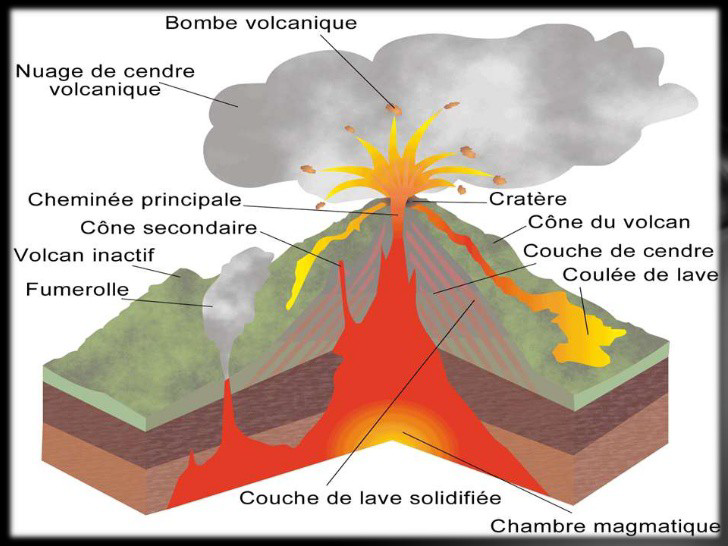
\includegraphics[width=.45\linewidth]{fig_01.png}
\caption{Schématisation d'un volcan en éruption \label{fig_01}}
\end{figure}


Avec ce constat, allié aux avancées technologiques dans le domaine de la robotique, la
Communauté Européenne a financé le projet ROBOVOLC dont le but était la réalisation d'un robot
mobile pour l'exploration volcanique. Ce robot devait être capable de :
\begin{itemize}
\item s'approcher d'un cratère actif ;
\item collecter des échantillons rocheux issus de rejets éruptifs ;
\item collecter des échantillons gazeux ;
\item collecter d'autres données physiques et chimiques.
\end{itemize}


\begin{obj}
Le sujet propose d'étudier quelques parties structurelles du système ROBOVOLC et de
valider plusieurs performances (liées à la mobilité et au prélèvement) de ce système. 
\end{obj}

\subsection{Présentation du système}


Le système ROBOVOLC est représenté sur la \autoref{fig_02}. Il se divise en plusieurs sous-systèmes
(liés à la navigation, au prélèvement et à la communication) qui sont détaillés dans les
diagrammes SysML fournis dans l'Annexe 1. 

\begin{figure}[H]
\centering
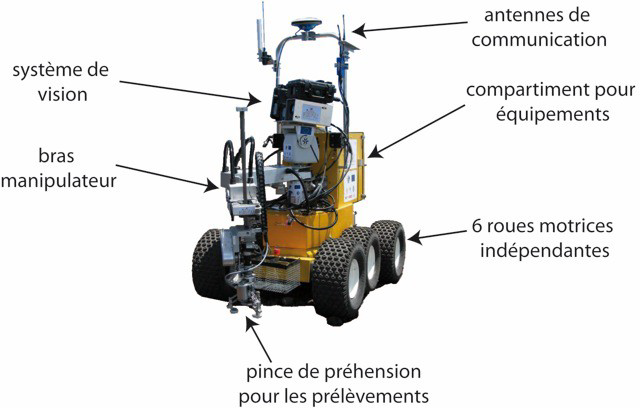
\includegraphics[width=.45\linewidth]{fig_02.png}
\caption{Représentation du système ROBOVOLC \label{fig_02}}
\end{figure}

La partie mécanique de ROBOVOLC est constituée de deux parties : (i) la plateforme (châssis,
roues) servant à la locomotion ; (ii) l'équipement d'analyse (bras manipulateur, pince, sondes) pour
le prélèvement et la mesure.

Une contrainte particulière dans la conception du système ROBOVOLC est qu'il est soumis à des
conditions extérieures particulièrement difficiles : terrain volcanique non structuré avec obstacles et
fortes pentes, températures très élevées près des zones éruptives (les gaz atteignent 600\degres C) mais
basses ailleurs à cause de l'altitude, présence de poussières de cendre très fines, ambiance
corrosive due aux composants acides, etc.


%Q1.1 : 
\question{Dans la phase de conception de ROBOVOLC, une alternative à un système de locomotion
à roues était un système volant. Donner deux inconvénients d'un tel système remettant en cause
son utilisation dans l'environnement volcanique considéré.}

ROBOVOLC est piloté à distance depuis un poste de contrôle (\autoref{fig_03}). La position géographique
du robot est obtenue par un système GPS et est envoyée au poste de contrôle par liaison radio.
De plus, l’opérateur peut visualiser en permanence les actions du système grâce aux images
transmises par une caméra embarquée.

L'énergie électrique nécessaire au système est apportée par une unité de puissance avec quatre
batteries couplées pour constituer deux unités de 24 V. La première est utilisée pour la plateforme,
l'autre pour l'équipement d'analyse. Ces batteries sont positionnées sur la partie basse du châssis.

%Q12
\question{Citer un intérêt à mettre les batteries en position basse sur le système.}


\begin{figure}[H]
\centering
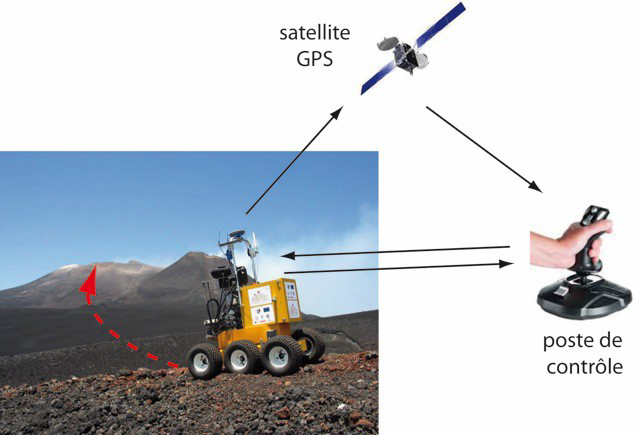
\includegraphics[width=.45\linewidth]{fig_03.png}
\caption{Illustration du pilotage à distance du système ROBOVOLC\label{fig_03}}
\end{figure}

Un cahier des charges partiel est donné ci-dessous :

\begin{center}
\begin{tabular}{ll}
\hline
\textbf{Critère} & \textbf{Valeur} \\ \hline \hline
Distance maximale entre ROBOVOLC et le poste de contrôle & \SI{2}{km} \\ \hline  
Temps de trajet pour une mission de 24 heures 		& \SI{1,5}{h} \\ \hline 
Vitesse de déplacement atteignable 				& \SI{0,5}{m/s} \\ \hline 
Dimensions du système (longueur/largeur/hauteur) 		& \SI{1900}{mm} x \SI{1200}{mm}x \SI{800}{mm}\\ \hline 
Masse maximale des composants modulaires 			& \SI{200}{kg} \\ \hline 
Charge utile maximale (instruments, etc.) 			& \SI{30}{kg} \\ \hline 
Pente maximale du sol 						& 40\degres \\ \hline 
Hauteur maximale d'un obstacle 					& \SI{400}{mm} \\ \hline 
Diamètre des objets à saisir entre 				& \SI{40}{mm} et \SI{300}{mm} \\ \hline 
Masse maximale des objets à saisir 				& \SI{2,5}{kg} \\ \hline 
\end{tabular}
\end{center}



%Q1.3 : 
\question{Citer une phase de vie du système qui contraint sa taille maximale et son poids maximal.}

La suite du sujet est composée de quatre parties qui étudient quelques particularités de la
structure mécanique du système ROBOVOLC :
\begin{itemize}
\item les parties \ref{sec_2} et \ref{sec_3} étudient la phase de déplacement (roulage) du système : la partie \ref{sec_2} vise
à valider les performances de mobilité et de suivi de trajectoire du système sur un sol plan
tandis que la partie \ref{sec_3} vise à valider les performances de franchissement d'obstacle sur un
terrain accidenté ;
\item les parties \ref{sec_4} et \ref{sec_5} étudient la phase de préhension d'échantillon : la partie \ref{sec_4} vise à valider
les performances du bras manipulateur tandis que la partie \ref{sec_5} vise à valider les
performances de la pince.
\end{itemize}



% 
% PARTIE 2
% 
\section{Étude de la mobilité sur un sol plan \label{sec_2}}


\begin{obj}
L'objectif de cette partie est de valider les performances de mobilité, de manoeuvrabilité et
de contrôle du système de locomotion de ROBOVOLC. On cherche notamment à vérifier le
critère suivant du cahier des charges :

\begin{center}
\begin{tabular}{ll}
\hline
\textbf{Critère} & \textbf{Valeur} \\ \hline \hline
Vitesse de déplacement atteignable &   \SI{0,5}{m/s} \\\hline
\end{tabular}
\end{center}

\end{obj}



%%%%%%%
%%%%%%%     PARTIE  2.2
%\subsection{Présentation du système de locomotion}
%
%\begin{obj}
%Dans cette sous-partie, on présente l'architecture du système de locomotion de
%ROBOVOLC.
%\end{obj}
%
%
%La plateforme de ROBOVOLC est équipée d'un châssis et de six roues motrices indépendantes et
%non directionnelles réparties symétriquement sur trois essieux (\autoref{fig_04}).
%
%
%\begin{figure}[H]
%\centering
%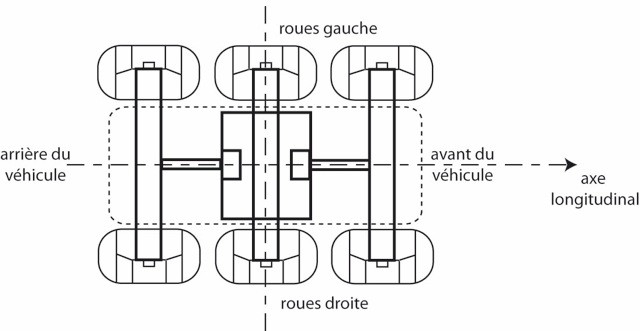
\includegraphics[width=.45\linewidth]{fig_04.png}
%\caption{Schématisation de la plateforme de ROBOVOLC (vue de dessus) \label{fig_04}}
%\end{figure}
%
%
%Chaque roue représente un module autonome (\autoref{fig_05}) dont la chaîne d'énergie est constituée
%d'une batterie, d'un variateur de vitesse, d'un moteur électrique à courant continu, d'un réducteur
%de vitesse (de rapport de réduction $r=\dfrac{1}{236}$, entouré sur la \autoref{fig_05}), d'un capteur de vitesse et
%d'un micro-contrôleur.
%Les roues sont équipées de pneumatiques spéciaux de diamètre extérieur $D=\SI{300}{mm}$.
%
%
%
%\begin{figure}[H]
%\centering
%\includegraphics[width=.45\linewidth]{fig_05w.png}
%\caption{Schéma de transmission de puissance pour chaque roue (vue de dessus) \label{fig_05}}
%\end{figure}
%
%
%On introduit le nombre (adimensionnel) de Froude $Fr=\dfrac{v}{\sqrt{gl_c}}$
%qui caractérise la vitesse de
%déplacement $v$ de ROBOVOLC relativement à sa taille caractéristique $l_c$ ; $g$ est l'accélération de la
%pesanteur. Lorsque $Fr>1$, les effets dynamiques ont une influence importante sur la trajectoire.
%
%%Q2.1 :
%\question{Montrer que les effets dynamiques peuvent être ici négligés.}
%
%Dans la suite de cette partie, on suppose un roulement sans glissement longitudinal au niveau du
%contact roue-sol. On suppose de plus que le sol est plan et horizontal, que le contact roue-sol est
%ponctuel, et que le châssis et les roues sont des solides indéformables.
%
%\subsection{Comportement en ligne droite}
%
%\begin{obj}
%Dans cette sous-partie, on détermine la commande permettant d'assurer une vitesse de
%déplacement en ligne droite donnée.
%\end{obj}
%
%Une modélisation de la plateforme est donnée sur la \autoref{fig_06}. On définit un repère local
%$\repere{O}{x}{y}{z}$ lié au châssis, $\vect{x}$ correspondant à l'axe longitudinal du châssis (appelé aussi ligne de
%foi) illustré sur la \autoref{fig_04}, et $\vect{z} correspondant à l'axe vertical. Le point $O$ est le centre
%géométrique et de masse de la plateforme dans le plan $\left({O},\vect{x}\vect{y}\right)$ parallèle au sol.
%
%Pour chaque roue notée $S_i$ ( $1\leq i \leq 6$), on définit :
%\begin{itemize}
%\item le point de contact $P_i$ entre la roue et le sol ;
%\item le point $O_i$ qui est la projection du point $P_i$ sur l'axe de rotation de la roue.
%\end{itemize}
%
%
%La position de chaque point $O_i$ est définie par $\vect{OO_i}=a_i \vect{x}  +e_i\vect{y}$ avec $a_i=\pm a$ et $e_i=\pm e$.
%Le châssis est noté $S_c$ et le sol est noté $S_0$.

%%%%%%%
%%%%%%%     PARTIE  2.2 PAS FINIE DE RECOPIER !!!!!!



\subsection{Technologie et asservissement en vitesse}
Dans cette sous-partie, on étudie l'asservissement en vitesse des roues en analysant la
technologie des composants et en déterminant les propriétés de comportement.
Chacune des roues dispose d'une motorisation indépendante avec un asservissement en vitesse.
Le contrôle de la vitesse de rotation de chaque roue permet de minimiser le glissement
longitudinal, notamment en mode automatique lorsque ROBOVOLC doit suivre un cap de manière
autonome.
Le système d'asservissement qui équipe chaque roue est destiné à contrôler sa vitesse de rotation
et doit permettre au système embarqué de détecter un glissement (manque d'adhérence). Ce
système est modélisé sur la \autoref{fig_07}.


\begin{figure}[H]
\centering
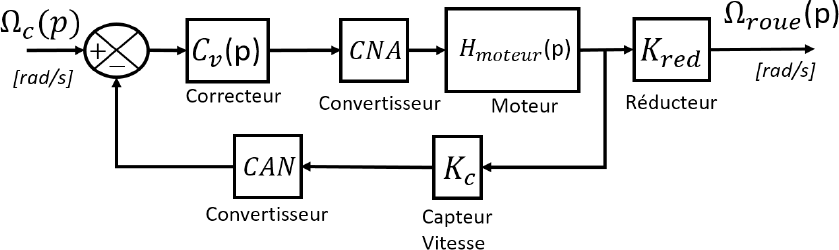
\includegraphics[width=.45\linewidth]{fig_07.png}
\caption{Structure d'asservissement \label{fig_07}}
\end{figure}




La fonction $K_c$ représente un capteur de vitesse permettant de mesurer la vitesse de rotation du
moteur.


%Q2.9 :
\question{Citer deux composants permettant de réaliser la fonction $K_c$ en précisant les
avantages/inconvénients et le type de signal (analogique ou numérique) en entrée/sortie de
chacun. Indiquer, en justifiant, la technologie la plus probablement retenue ici.}

\subsubsection{Étude du convertisseur numérique-analogique (CNA)}

La valeur$U (t)$ en entrée du CNA est codée sous forme d'un entier non signé sur 16 bits. Elle est
ensuite convertie en grandeur analogique $\indice{U}{mot}$ entre $-\SI{10}{V}$ et $6\SI{10}{V}$ pour $U (t)$ évoluant en
hexadécimal de 0000 à sa valeur maximale FFFF.

%Q2.10 :
\question{Donner la valeur numérique de $U (t)$ à appliquer pour obtenir une valeur nulle en sortie
du CNA. A quelle consigne correspond la valeur hexadécimale d'entrée $U (t) =\text{A000}$?}

\subsubsection{Étude du convertisseur analogique-numérique (CAN)}

Le capteur utilisé pour mesurer la vitesse de rotation est de type dynamo-tachymétrique, ce choix
répondant aux exigences de tenue en température et robustesse. Le capteur fournit une tension
directement proportionnelle à la vitesse de rotation de la roue, cette tension variant au maximum
entre $-\SI{610}{mV}$ et $+\SI{650}{mV}$. Le CAN employé possède plusieurs canaux de conversion A/N 12 bits
d'une linéarité de +/-1 bit. Le temps de conversion par canal est de 25 micro-secondes.

%Q2.11 :
\question{Calculer la résolution en mV du CAN.}


%Q2.12 :
\question{Donner les deux hypothèses principales qu’il faut faire pour pouvoir utiliser un modèle de
système linéaire continu invariant.}

\subsubsection{Asservissement en vitesse}

On suppose dans la suite que :
\begin{itemize}
\item $C_v ( p)=K_v$ (constante) ;
\item $K_c =1$ (gain de capteur) ;
\item  les blocs CAN et CNA sont modélisés par des blocs unitaires.
\end{itemize}

La\autoref{fig_08} représente la réponse mesurée du moteur lorsqu’un échelon unitaire de tension est
envoyé en entrée.



%Q2.13 : 
\question{Exprimer par un modèle du premier ordre sous forme canonique la fonction de transfert
$\indice{H}{moteur}( p)$ du moteur, et identifier ses paramètres.}

%Q2.14 : 
\question{Calculer la fonction de transfert $\dfrac{\indice{\Omega}{roue}( p)}{\Omega_c(p)}$ sous forme canonique.}

%Q2.15 : 
\question{Exprimer les conditions pour avoir des valeurs d'erreur statique en position et en vitesse
inférieures à 1\%. Proposer un moyen d'obtenir ces erreurs statiques nulles.}


%% Partie 2.5 TODO
%\subsection{Maîtrise de trajectoire}









Les éruptions volcaniques peuvent avoir un impact important sur l'activité humaine, provoquant à
la fois des déplacements de population, des dégâts matériels, ainsi que des changements de
topographie et de climat. On considère qu'actuellement 10\% de la population terrestre vit sous la
menace des volcans, et 1500 volcans potentiellement en activité sont répertoriés sur la planète.
Par conséquent, une compréhension fine des phénomènes volcaniques et une meilleure maîtrise
des risques associés constituent un enjeu scientifique majeur.

Les observations scientifiques réalisées pendant les phases éruptives sont aujourd'hui
fondamentales pour l'étude des volcans. En effet, les prélèvements des gaz magmatiques et des
échantillons rocheux rejetés lors de ces phases constituent des indicateurs fiables de l'activité
interne des volcans ; ils sont donc une riche source d'informations pour les volcanologues.
Cependant, les phases éruptives sont aussi des phases actives très dangereuses et il est
primordial de limiter les risques humains lors d'observations et de prélèvements à proximité des
cratères en éruption (\autoref{fig_01}). 



\begin{figure}[H]
\centering
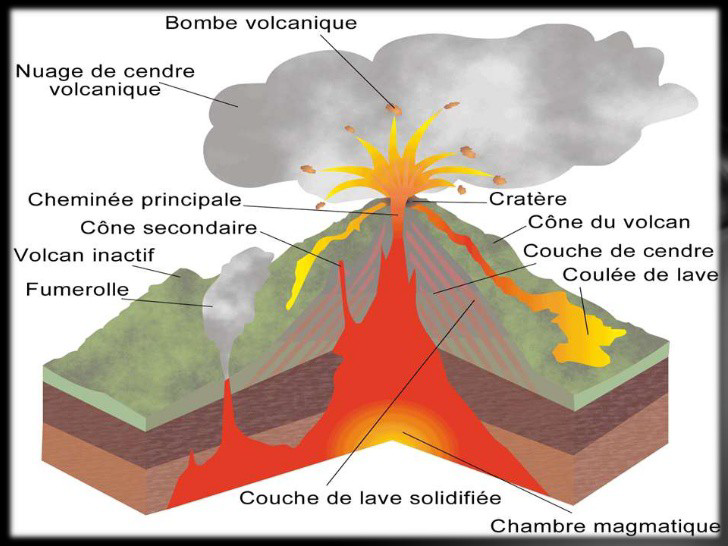
\includegraphics[width=.45\linewidth]{fig_01.png}
\caption{Schématisation d'un volcan en éruption \label{fig_01}}
\end{figure}


Avec ce constat, allié aux avancées technologiques dans le domaine de la robotique, la
Communauté Européenne a financé le projet ROBOVOLC dont le but était la réalisation d'un robot
mobile pour l'exploration volcanique. Ce robot devait être capable de :
\begin{itemize}
\item s'approcher d'un cratère actif ;
\item collecter des échantillons rocheux issus de rejets éruptifs ;
\item collecter des échantillons gazeux ;
\item collecter d'autres données physiques et chimiques.
\end{itemize}


\begin{obj}
Le sujet propose d'étudier quelques parties structurelles du système ROBOVOLC et de
valider plusieurs performances (liées à la mobilité et au prélèvement) de ce système. 
\end{obj}

\subsection{Présentation du système}


Le système ROBOVOLC est représenté sur la \autoref{fig_02}. Il se divise en plusieurs sous-systèmes
(liés à la navigation, au prélèvement et à la communication) qui sont détaillés dans les
diagrammes SysML fournis dans l'Annexe 1. 

\begin{figure}[H]
\centering
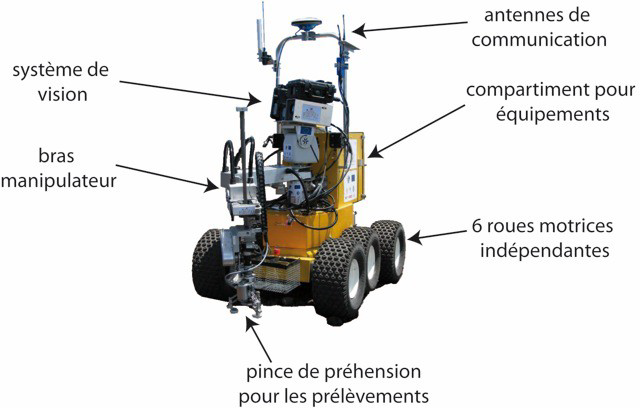
\includegraphics[width=.45\linewidth]{fig_02.png}
\caption{Représentation du système ROBOVOLC \label{fig_02}}
\end{figure}

La partie mécanique de ROBOVOLC est constituée de deux parties : (i) la plateforme (châssis,
roues) servant à la locomotion ; (ii) l'équipement d'analyse (bras manipulateur, pince, sondes) pour
le prélèvement et la mesure.

Une contrainte particulière dans la conception du système ROBOVOLC est qu'il est soumis à des
conditions extérieures particulièrement difficiles : terrain volcanique non structuré avec obstacles et
fortes pentes, températures très élevées près des zones éruptives (les gaz atteignent 600\degres C) mais
basses ailleurs à cause de l'altitude, présence de poussières de cendre très fines, ambiance
corrosive due aux composants acides, etc.


%Q1.1 : 
\question{Dans la phase de conception de ROBOVOLC, une alternative à un système de locomotion
à roues était un système volant. Donner deux inconvénients d'un tel système remettant en cause
son utilisation dans l'environnement volcanique considéré.}

ROBOVOLC est piloté à distance depuis un poste de contrôle (\autoref{fig_03}). La position géographique
du robot est obtenue par un système GPS et est envoyée au poste de contrôle par liaison radio.
De plus, l’opérateur peut visualiser en permanence les actions du système grâce aux images
transmises par une caméra embarquée.

L'énergie électrique nécessaire au système est apportée par une unité de puissance avec quatre
batteries couplées pour constituer deux unités de 24 V. La première est utilisée pour la plateforme,
l'autre pour l'équipement d'analyse. Ces batteries sont positionnées sur la partie basse du châssis.

%Q12
\question{Citer un intérêt à mettre les batteries en position basse sur le système.}


\begin{figure}[H]
\centering
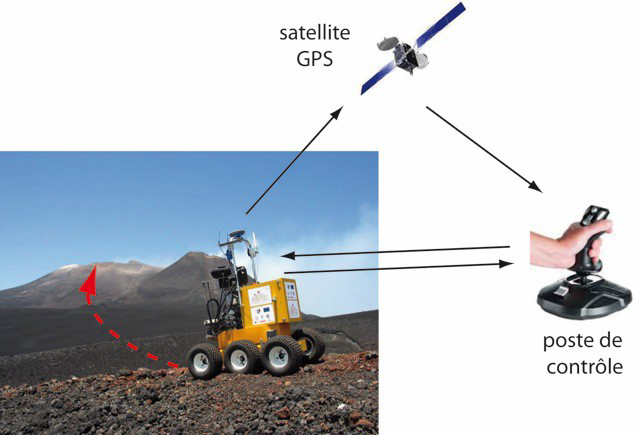
\includegraphics[width=.45\linewidth]{fig_03.png}
\caption{Illustration du pilotage à distance du système ROBOVOLC\label{fig_03}}
\end{figure}

Un cahier des charges partiel est donné ci-dessous :

\begin{center}
\begin{tabular}{ll}
\hline
\textbf{Critère} & \textbf{Valeur} \\ \hline \hline
Distance maximale entre ROBOVOLC et le poste de contrôle & \SI{2}{km} \\ \hline  
Temps de trajet pour une mission de 24 heures 		& \SI{1,5}{h} \\ \hline 
Vitesse de déplacement atteignable 				& \SI{0,5}{m/s} \\ \hline 
Dimensions du système (longueur/largeur/hauteur) 		& \SI{1900}{mm} x \SI{1200}{mm}x \SI{800}{mm}\\ \hline 
Masse maximale des composants modulaires 			& \SI{200}{kg} \\ \hline 
Charge utile maximale (instruments, etc.) 			& \SI{30}{kg} \\ \hline 
Pente maximale du sol 						& 40\degres \\ \hline 
Hauteur maximale d'un obstacle 					& \SI{400}{mm} \\ \hline 
Diamètre des objets à saisir entre 				& \SI{40}{mm} et \SI{300}{mm} \\ \hline 
Masse maximale des objets à saisir 				& \SI{2,5}{kg} \\ \hline 
\end{tabular}
\end{center}



%Q1.3 : 
\question{Citer une phase de vie du système qui contraint sa taille maximale et son poids maximal.}

La suite du sujet est composée de quatre parties qui étudient quelques particularités de la
structure mécanique du système ROBOVOLC :
\begin{itemize}
\item les parties \ref{sec_2} et \ref{sec_3} étudient la phase de déplacement (roulage) du système : la partie \ref{sec_2} vise
à valider les performances de mobilité et de suivi de trajectoire du système sur un sol plan
tandis que la partie \ref{sec_3} vise à valider les performances de franchissement d'obstacle sur un
terrain accidenté ;
\item les parties \ref{sec_4} et \ref{sec_5} étudient la phase de préhension d'échantillon : la partie \ref{sec_4} vise à valider
les performances du bras manipulateur tandis que la partie \ref{sec_5} vise à valider les
performances de la pince.
\end{itemize}



% 
% PARTIE 3
% 
\section{Étude du comportement sur terrain accidenté \label{sec_3}}
\ifprof\else
Le terrain volcanique est en pratique très accidenté, avec la présence d'obstacles (roches) et de
fortes pentes (\autoref{fig_10}). Par conséquent, le système de locomotion de ROBOVOLC doit être
adapté à ce type de terrain.
\fi
\begin{obj}
L'objectif de cette partie est de valider les performances d'agilité et de franchissement
d'obstacle du système sur des terrains non structurés avec difficultés topologiques
(pentes, obstacles). On souhaite vérifier les critères suivants du cahier des charges :
\begin{center}
\begin{tabular}{ll}
\hline
\textbf{Critère} & \textbf{Valeur} \\ \hline \hline
Masse maximale des composants modulaires & \SI{200}{kg}\\ 
Pente maximale du sol & 40\degres \\ 
Hauteur maximale d'un obstacle & \SI{400}{mm} \\ 
\hline
\end{tabular}
\end{center}
\end{obj}
\ifprof\else
Dans toute cette partie, les effets dynamiques sont négligés et on se place en statique.


\begin{figure}[H]
\centering
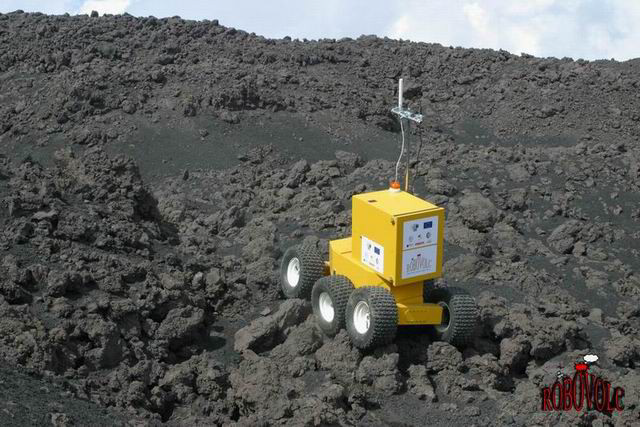
\includegraphics[width=.45\linewidth]{fig_10.png}
\caption{Illustration du comportement de ROBOVOLC sur terrain accidenté \label{fig_10}}
\end{figure}
\fi

\subsection{Modélisation du châssis}

\begin{obj}
Dans cette sous-partie, on établit un modèle statique du châssis de ROBOVOLC.
\end{obj}
\ifprof\else
La mobilité sur terrain accidenté est obtenue, en plus de par la motorisation indépendante des
roues, par l'utilisation d'un châssis articulé. Celui-ci a une structure tubulaire avec des articulations
passives (non actionnées) permettant à ROBOVOLC de s'adapter à toute surface non plane. Une
illustration des cinq mouvements indépendants permis par les articulations est donnée sur la
\autoref{fig_11}.

\begin{figure}[H]
\centering
\begin{tabular}{|p{.3\linewidth}|p{.3\linewidth}|p{.3\linewidth}|}
\hline
Châssis au repos & Mouvement 1 : rotation de l'essieu avant
autour de l'axe longitudinal & Mouvement 2 :
rotation de l'essieu central
autour de l'axe longitudinal \\ \hline
\begin{center}
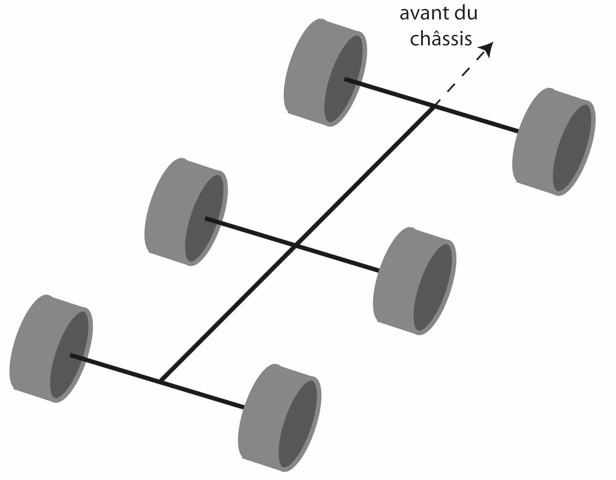
\includegraphics[width=.9\linewidth]{fig_11_a.png}
\end{center}
&
\begin{center}
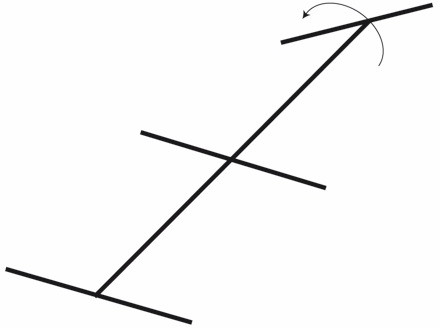
\includegraphics[width=.9\linewidth]{fig_11_b.png}
\end{center}
&
\begin{center}
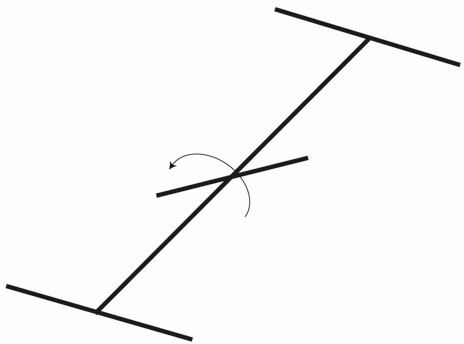
\includegraphics[width=.9\linewidth]{fig_11_c.png}
\end{center} \\ \hline
Mouvement 3 :
rotation de l'essieu arrière
autour de l'axe longitudinal & 
Mouvement 4 :
rotation de l'arbre avant
autour de l'axe transversal &
Mouvement 5 :
rotation de l'arbre arrière
autour de l'axe transversal \\ \hline
\begin{center}
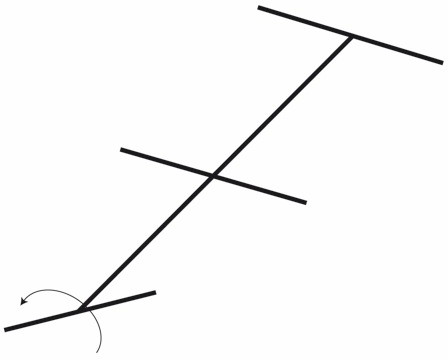
\includegraphics[width=.9\linewidth]{fig_11_d.png}
\end{center}
&
\begin{center}
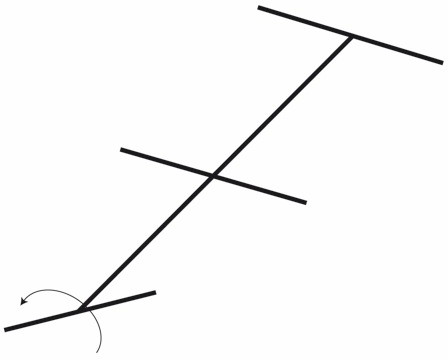
\includegraphics[width=.9\linewidth]{fig_11_e.png}
\end{center}
&
\begin{center}
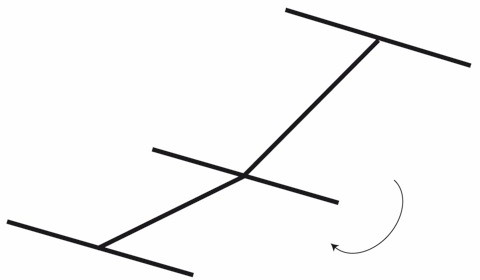
\includegraphics[width=.9\linewidth]{fig_11_f.png}
\end{center} \\ \hline
\end{tabular}

\caption{Illustration des mouvements de déformation du châssis\label{fig_11}}
\end{figure}

Le châssis est composé de cinq parties orientables les unes par rapport aux autres (\autoref{fig_12}) :
\begin{itemize}
\item l'essieu avant, noté EAV, reliant les roues avant 1 et 2 ;
\item l'essieu central, noté EC, reliant les roues centrales 3 et 4 ;
\item l'essieu arrière, noté EAR, reliant les roues arrière 5 et 6 ;
\item l'arbre avant, noté AAV, connectant les essieux EAV et EC ;
\item l'arbre arrière, noté AAR, connectant les essieux EC et EAR.
\end{itemize}
On rappelle que l'empattement entre deux essieux successifs est noté $a$, et que la distance entre
deux roues d'un même essieu est notée $2e$.
Les différentes parties sont reliées entre elles par des articulations possédant une raideur en
rotation imposée. Par la suite, on supposera cette raideur négligeable devant les autres actions
mécaniques mises en jeu.
Un schéma cinématique de la plateforme (châssis+roues) est présenté sur la \autoref{fig_12}.

\begin{figure}[H]
\centering
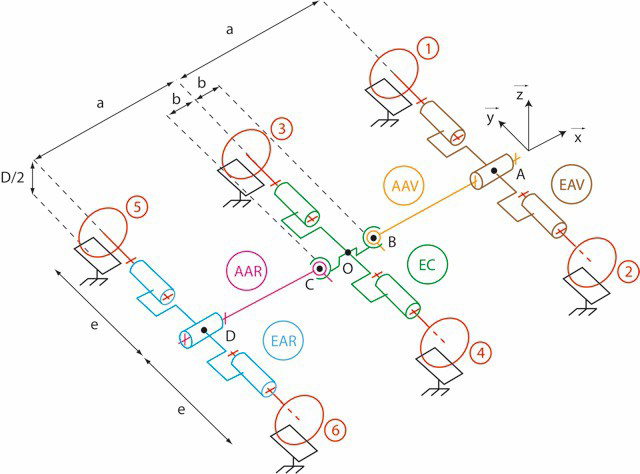
\includegraphics[width=.65\linewidth]{fig_12.png}
\caption{Schéma cinématique de la plateforme\label{fig_12}}
\end{figure}

Les deux articulations EC-AAV et EC-AAR, situées à une distance longitudinale $\pm b$ de l'essieu
EC, autorisent une rotation selon les directions $\vect{x}$ et $\vect{y}$; elles sont modélisées par des liaisons
rotule à doigt de centres respectifs $B$ et $C$. Les deux articulations EAV-AAV et EAR-AAR
autorisent une rotation selon la direction $\vect{x}$ seulement ; elles sont modélisées par des liaisons
pivot d'axe $\axe{O}{x}$.

D'autre part, les six liaisons essieu-roue sont modélisées par des liaisons pivot d'axe $\axe{A}{y}$
(roues avant), $\axe{O}{y}$ (roues centrales) ou $\axe{D}{y}$ (roues arrière). De plus, le contact de chaque
roue i avec le sol est modélisé en première approche par une liaison ponctuelle de normale
$\axe{P_i}{z}$.

On considère dans les questions \ref{q3.1} et \ref{q3.2} que les liaisons sont parfaites sans frottements.

\fi

\question{ \label{q3.1} Déterminer le nombre de mobilités du modèle du système.}
\ifprof
\begin{corrige}\textbf{ -- UPSTI}\\ 
\vspace{-.7cm}
\begin{itemize}
\item 6 mobilités : 6 pivots de roues liées à la rotation des roues par rapport à leur axe.
\item Liaison appui plan de l’ensemble par rapport au sol et donc 2 translations et une rotation de l’ensemble par rapport au sol : 3 mobilités.
\item Rotations en Rz des ensembles AAV ou AAR par rapport à EC : 2 mobilités
\item Rotations simultanées de AAR et AAV par rapport à EC en Ry . (Une seule mobilité)
\end{itemize}
Au total : 12 mobilités. 
\end{corrige}
\else
\fi

\question{ \label{q3.2} Montrer que le modèle est isostatique. Conclure quant à la capacité du châssis à maintenir les roues au contact du sol en toute circonstance.}
\ifprof
\begin{corrige}\textbf{ -- UPSTI}\\ 
\vspace{-.3cm}
\begin{multicols}{2}
On peut utiliser ici directement les formules de calcul du degré d’hyperstatisme.
En calculant à partir des relations cinématiques :
\begin{itemize}
\item Nombre cyclomatique $\mu =16-12+1=5$
\item Nombre de mobilités $m=12$
\item Inconnues cinématiques $I_c=6\times 5+2\times 2+8\times 1=42$
\end{itemize}
Le degré d’hyperstatisme est donc égal à : $h=12+30-42=0$.
Le système est isostatique.

En calculant à partir des inconnues de statique :
\begin{itemize}
\item Nombre de pièces  $p=12$.
\item Nombre de mobilités $m=12$.
\item Inconnues cinématiques $I_S=6\times 1+2\times 4+8\times 5=54$.
\end{itemize}
Le degré d’hyperstatisme est donc égal à : $h=12-66+54=0$.

Le système est isostatique

\end{multicols}
\end{corrige}
\else
\fi

\question{ \label{q3.3} Proposer un modèle de liaison parfaite pour le contact roue-sol qui permet de tenir compte, dans une étude de statique sans glissement, du frottement longitudinal et transversal. Peut-on calculer toutes les inconnues statiques de liaison dans ce cas ?}
\ifprof
\begin{corrige}\textbf{ -- UPSTI}\\ 
La liaison parfaite qui permet de tenir en compte dans une étude de statique sans glissement  à la fois des efforts normaux, du frottement longitudinal et du frottement transversal est une liaison rotule. Il faudrait alors modéliser les 6 contacts entre les roues et le sol par des liaisons rotule pour résoudre.


\textbf{Dans ce cas, le degré d’hyperstatisme est modifié :}

12 inconnues de liaison sont supprimées, mais seule une mobilité (rotations simultanées autour de AAC et AAV autour de EC) subsiste. Le système est hyperstatique de degré 1 et toutes les inconnues de statique ne peuvent être déterminées. 

\end{corrige}
\else
\fi

\ifprof\else
On considère par la suite que le sol est horizontal dans la direction $\vect{y}$; on se ramène alors à un
problème dans le plan médian $\left(O,\vect{x},\vect{z}\right)$. Dans cette configuration plane, la plateforme est
constituée de trois ensembles articulés pour s'adapter au terrain accidenté (\autoref{fig_13}) :
\begin{itemize}
\item l'ensemble avant (noté ENSAV) constitué des pièces EAV, AAV et des roues 1 et 2 ;
\item l'ensemble central (noté ENSC) constitué de la pièce EC et des roues 3 et 4 ;
\item l'ensemble arrière (noté ENSAR) constitué des pièces EAR, AAR et des roues 5 et 6.
\end{itemize}

On considère qu'il y a roulement sans glissement au contact roue-sol. Les actions mécaniques du
sol sur chaque ensemble sont schématisées sur la \autoref{fig_13}; elles sont modélisées par un effort
normal ($\indice{N}{AV}$, $\indice{N}{C}$ ou $\indice{N}{AR}$) et un effort tangentiel de traction ($\indice{T}{AV}$, $\indice{T}{C}$ ou $\indice{T}{AR}$) appliqués aux
points $\indice{P}{AV}$, $\indice{P}{C}$ ou $\indice{P}{AR}$ (projections des points de contact roue-sol $P_i$ dans le plan médian $\left(O,\vect{x},\vect{z}\right)$).

\begin{figure}[H]
\centering
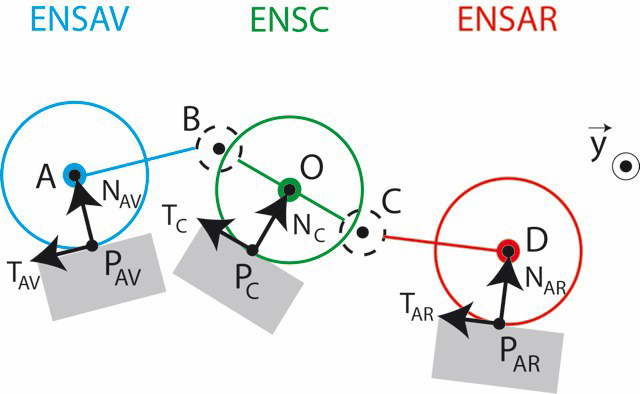
\includegraphics[width=.45\linewidth]{fig_13.png}
\caption{Configuration plane du châssis\label{fig_13}}
\end{figure}
\fi

\question{Indiquer s'il est possible de déterminer, par une analyse statique globale, les différentes
actions $\indice{N}{AV}$, $\indice{T}{AV}$, $\indice{N}{C}$, $\indice{T}{C}$, $\indice{N}{AR}$, $\indice{T}{AR}$. Justifier la réponse.}

\ifprof\else
La modélisation plane de la \autoref{fig_13} est considérée dans la suite de cette partie.
\fi

\subsection{Comportement en pente et stabilité}
\begin{obj}
Dans cette sous-partie, on analyse le comportement en pente et la stabilité statique de la
plateforme.
\end{obj}
\ifprof\else
On considère ici un sol plan dans le plan $\left(O,\vect{x},\vect{z}\right)$ et incliné d'un angle $\alpha$ par rapport à
l'horizontale (\autoref{fig_14}). La masse totale du système ROBOVOLC est répartie sur les trois
ensembles de la plateforme; les ensembles ENSAV et ENSAR ont la même masse
$\indice{m}{AV}=\indice{m}{AR}=m$ tandis que l'ensemble ENSC a une masse $m_C=M$. Les centres de gravité des
trois ensembles sont notés respectivement $\indice{G}{AV}$, $\indice{G}{C}$ et $\indice{G}{AR}$ ; ils sont indiqués sur la \autoref{fig_14}.

On a : $\vect{\indice{AG}{AV}}=\vect{\indice{OG}{C}}=\vect{\indice{DG}{AR}}=h\vect{z}$. 
Toutes les roues ont le même diamètre noté $D$.
On donne $D =\SI{300}{mm}$, $m =\SI{60}{kg}$, $M =\SI{80}{kg}$, $a =\SI{800}{mm}$, $b =\SI{200}{mm}$, $h =\SI{450}{mm}$.


\begin{figure}[H]
\centering
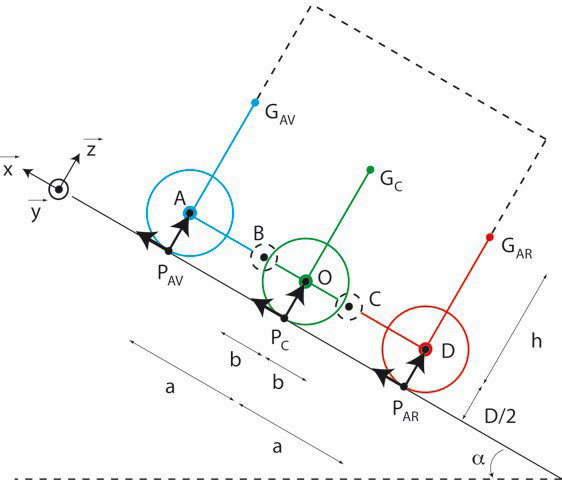
\includegraphics[width=.45\linewidth]{fig_14.png}
\caption{Configuration en pente \label{fig_14}}
\end{figure}

\fi

\question{Dans la configuration $\alpha = 0\degres$ (pente nulle), justifier la répartition des efforts normaux suivante :  $\indice{N}{AV}= \indice{N}{AR}=mg$, $N_C=Mg$.}
\ifprof
\begin{corrige}\textbf{ -- UPSTI}\\ 
Par symétrie du système, on peut commencer par remarquer que le centre de gravité du système est situé en $G_c$.

On isole tout l’ensemble en équilibre et on applique le Principe Fondamental de Statique. 

Le Théorème de la Résultante est projeté sur $\vect{z}$. Le Théorème du Moment Statique est appliqué au point $P_c$ en projection sur $\vect{y}$.

On obtient alors les relations suivantes :
$\left\{
\begin{array}{l}
\indice{N}{AV} +\indice{N}{C}+\indice{N}{AR}-(M+2m)g=0 \\
a\indice{N}{AV} - a\indice{N}{AR} = 0 . \\
\end{array}
\right.$
Ensuite, par identification, on obtient $\indice{N}{AV}=\indice{N}{AR}=mg$ et $N_C = Mg$.

\end{corrige}
\else
\fi

\question{Déterminer, en fonction des données géométriques, la hauteur $h$ limite des centres de
gravité avant basculement du système sur une pente inclinée d'un angle $\alpha$. En déduire la valeur limite de $h$ à respecter pour satisfaire le cahier des charges, puis faire l'application numérique et conclure. On donne $\tan 50\degres \simeq 1,2$.}
\ifprof
\begin{corrige}\textbf{ -- UPSTI}\\ 
On commence par étudier les configurations possibles de basculement :
\begin{itemize}
\item Basculement de ENSAV autour de B.
\item Basculement de ENSAV et ENSC simultanément.
\end{itemize}


Le basculement débutera donc obligatoirement par le basculement de la partie avant du véhicule.
A l’aide de considérations graphiques, il est possible de dire que le basculement débutera lorsque les efforts de pesanteur sur ENSAV seront « à droite » de B.
 
La situation limite de basculement est tracée ci-contre (l’effort de pesanteur passe par le point $B$).
On lit directement sur la figure en utilisant les données du schéma :
$\tan\alpha = \dfrac{AB}{\indice{AG}{AV}} = \dfrac{a-b}{h}$.

La hauteur limite des centres de gravité avant basculement dans une pente $\alpha$ est donc :
$\indice{h}{lim}=\dfrac{a-b}{\tan \alpha}$.

Le cahier des charges impose de monter des pentes de 50\degres, on obtient donc une hauteur limite $h$ après application numérique : $\indice{h}{lim}=0.6/1.2=\SI{0,5}{m}$.

\textbf{Deuxième méthode : }
En isolant ENSAV et en appliquant le Principe Fondamental de la Statique, on pourra résoudre sachant qu’à la limite du basculement, $\indice{N}{AV}$ est connu et vaut 0.

\begin{itemize}
\item Théorème de la résultante sur $\vect{x}$ : $\indice{T}{AV}+X_{\text{ensc-ensav}}-mg \sin \alpha = 0$
\item Théorème de la résultante sur $\vect{z}$ : $\indice{N}{AV}+Y_{\text{ensc-ensav}}-mg \cos \alpha = 0$.
\item Théorème du Moment sur $\vect{y}$ au point $B$ : $ -mgh \sin \alpha +  mg(a-b) \cos\alpha \indice{N}{AV} (a-b)- \indice{T}{AV} h=0$.
\end{itemize}

À la limite du basculement, les efforts sur la roue avant sont nuls et l’équation de moment devient :
$-mg\indice{h}{lim} +mg(a-b) \cos\alpha = 0$ soit encore $\indice{h}{lim} = \dfrac{a-b}{\tan \alpha}$.
\end{corrige}
\else
\fi


\ifprof
Dans la question suivante, on fait l'hypothèse (notée HYP1) de limite de glissement au contact
entre le sol et la paire de roues de l'ensemble ENSC le plus chargé. On note $\mu$ le coefficient
de frottement.
\else
\fi

\question{Montrer que l'hypothèse HYP1 permet de calculer l'ensemble des efforts de contact roue-sol dans la configuration $\alpha \neq 0$ (le calcul n'est pas demandé). Quelle équation permet de démontrer que $\indice{N}{AV}\neq\indice{N}{AR}$ dans cette configuration ?}
\ifprof
\begin{corrige}\textbf{ -- UPSTI}\\ 
Dans le cas où les 3 coefficients de frottement ne sont pas connus, on a démontré qu’il n’était pas possible de résoudre, car il nous manquait une équation.
Avec l’HYP1, la résolution devient possible puisque l’on rajoute une équation de comportement.
L’écriture du Théorème du Moment Statique appliqué au point $P_c$  permet de démontrer l’inégalité $\indice{N}{AV}\neq \indice{N}{AR}$.

\end{corrige}
\else
\fi

\subsection{Franchissement d'un obstacle}

\begin{obj}
Dans cette sous-partie, on étudie le franchissement par ROBOVOLC d'un obstacle en
analysant les différentes phases du franchissement en terme d'efforts sur les roues.
\end{obj}
\ifprof\else
L'obstacle est matérialisé par une marche (pente verticale) de hauteur $H$ dans le plan $\left(O,\vect{x},\vect{z}\right)$,
$\vect{z}$ correspondant à la verticale \autoref{fig_15}.
On s'intéresse particulièrement aux trois phases représentées sur la \autoref{fig_15}, correspondant à la
montée de chacun des trois ensembles (respectivement ENSAV pour la phase 1, ENSC pour la
phase 2 et ENSAR pour la phase 3) le long de l'obstacle.

Les notations utilisées (géométrie, actions mécaniques) sont similaires à celles de la sous-partie
précédente.

\begin{figure}[H]
\centering
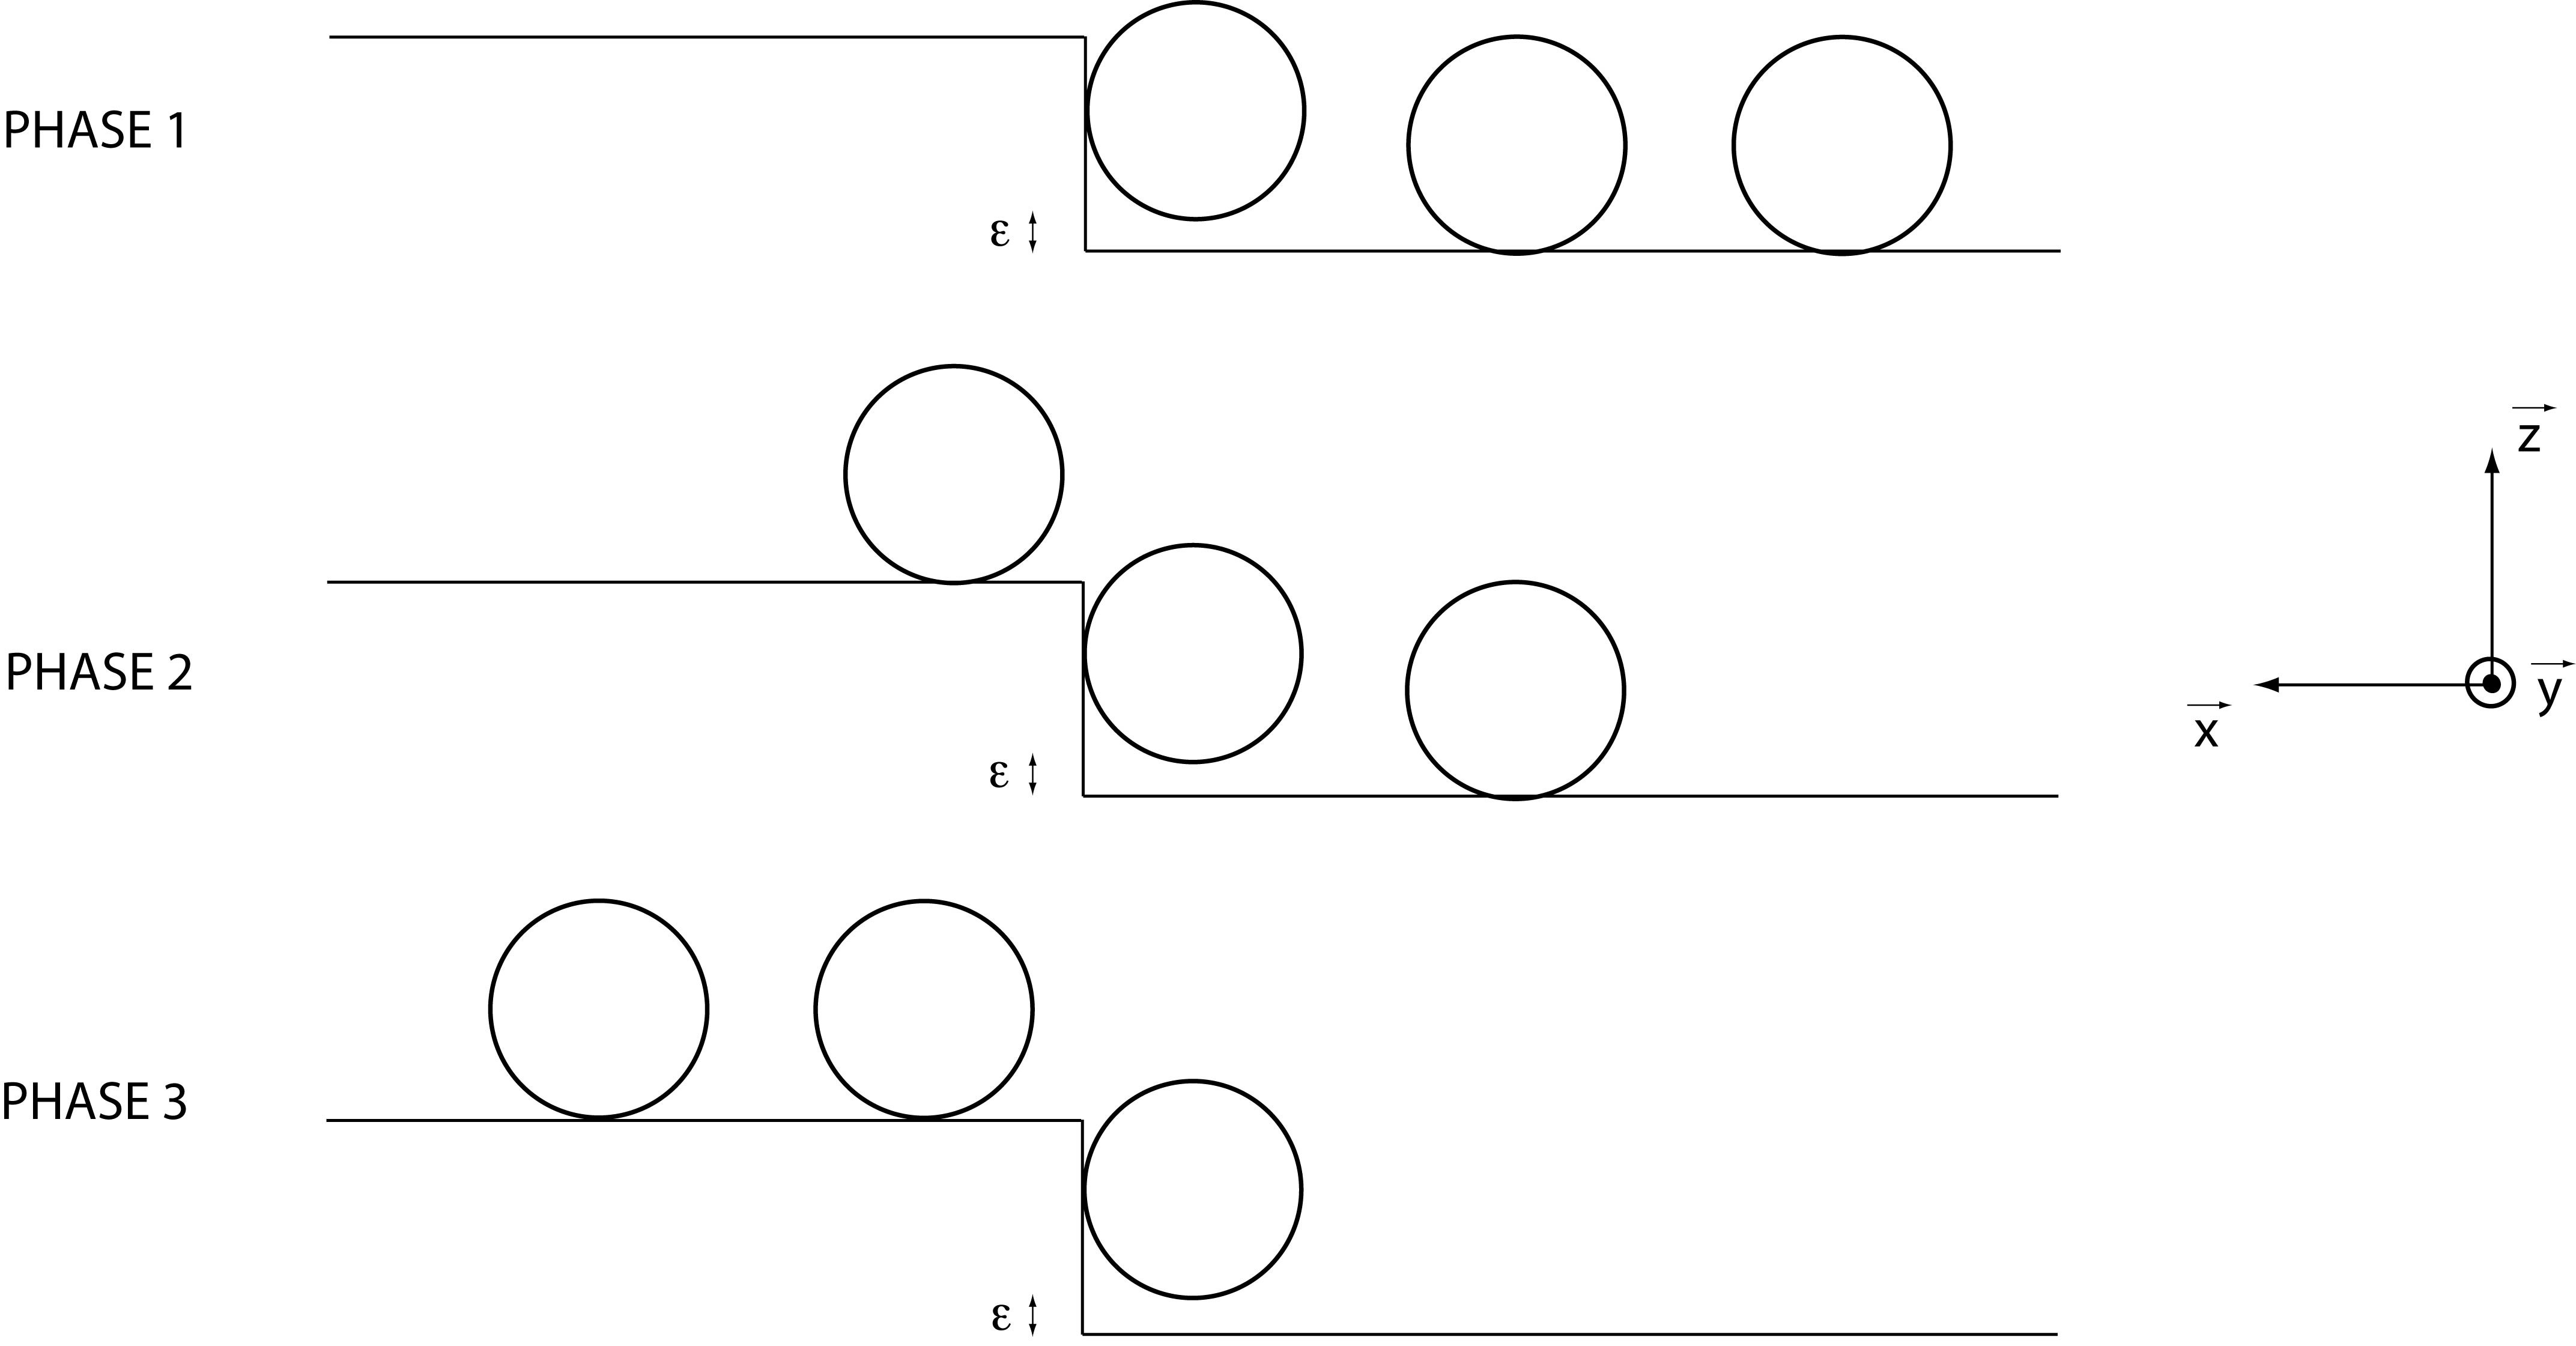
\includegraphics[width=.45\linewidth]{fig_15.png}
\caption{Schématisation de l'obstacle et des phases de son franchissement\label{fig_15}}
\end{figure}
\fi


% Q3.8
\question{Pour chacune des trois phases, donner les deux équations obtenues par le théorème de la
résultante statique selon $\vect{x}$ et $\vect{z}$. Les autres équations de statique ne sont pas demandées.}
\ifprof
\begin{corrige}\textbf{ -- UPSTI}\\ 
\begin{itemize}
\item \textbf{Phase 1} : 
\begin{itemize} 
\item TRS en $\vect{x}$ : $-\indice{N}{AV}+T_C+\indice{T}{AR}=0$
\item TRS en $\vect{z}$ : $\indice{T}{AV}+N_C+\indice{N}{AR}-\left(2m + M\right)g=0$
\end{itemize}
\item \textbf{Phase 2} : 
\begin{itemize} 
\item TRS en $\vect{x}$ : $\indice{T}{AV}-N_C+\indice{T}{AR}=0$
\item TRS en $\vect{z}$ : $\indice{N}{AV}+T_C+\indice{N}{AR}-\left(2m + M\right)g=0$
\end{itemize}
\item \textbf{Phase 3} : 
\begin{itemize} 
\item TRS en $\vect{x}$ : $\indice{T}{AV}+T_C-\indice{N}{AR}=0$
\item TRS en $\vect{z}$ : $\indice{N}{AV}+N_C+\indice{T}{AR}-\left(2m + M\right)g=0$
\end{itemize}
\end{itemize}
\end{corrige}
\else
\fi

\ifprof
\else
Sous l'hypothèse (notée HYP2) de \textbf{limite de glissement pour la paire de roues montant le long de l'obstacle}, l'ensemble des équations de statique donne accès aux valeurs des efforts de contact roue-sol. On représente dans l'Annexe 2 les diagrammes d'évolution simulée de ces efforts au cours du franchissement de l'obstacle, pour une hauteur de l'obstacle $H =\SI{400}{mm}$ et un coefficient de frottement roue-sol $\mu = 0,5$ ou $\mu = 2$.
\fi

% Q3.9
\question{Identifier les plages temporelles des diagrammes où ont lieu chacune des phases 1, 2 et 3.
Indiquer également à quoi correspondent les autres phases des diagrammes, et préciser l'origine
des sauts d'effort observés.}
\ifprof
\begin{corrige}\textbf{ -- UPSTI}\\ 
Pour $t\in [1;2]$ s : phase 1 ; pour $t\in [3;4]$ s :  Phase 2 ; Pour $t\in [5;6]$ s : Phase 3.
Remarque : Une erreur s’est glissée dans le document Annexe 2. Il faut lire µ=2, et non 0,2.
Les autres phases correspondent à des états transitoires lorsqu’aucune roue ne touche les marches verticales.
\end{corrige}
\else
\fi

% Q3.10
\question{Expliquer pourquoi, sous l'hypothèse HYP2, il n'est pas possible de franchir l'obstacle
avec un coefficient de frottement $\mu = 0,5$.}
\ifprof
\begin{corrige}\textbf{ -- UPSTI}\\ 
Avec l’hypothèse $\mu = 0,5$, la condition sur la roue avant et sur la roue arrière entre 3 et \SI{4}{s} impose $\indice{T}{AV}  > 0,5 \cdot  \indice{N}{AV}$  et $\indice{T}{AR} > 0,5 \times \indice{N}{AR}$, ce qui est impossible. Donc, il n’est pas possible de franchir l’obstacle avec un tel coefficient de frottement.
\end{corrige}
\else
\fi


\subsection{Sélection des couples optimaux}

\begin{obj}
Dans cette sous-partie, on met en place un algorithme de calcul des couples optimaux à
appliquer à chaque roue.
\end{obj}

\ifprof\else
Les actions extérieures exercées sur chaque roue (ou chaque paire de roues) sont représentées
sur la \autoref{fig_16} :
\begin{itemize}
\item $N$ est la composante d'effort normale au contact roue-sol ;
\item $T$ est la composante d'effort tangentielle au contact roue-sol ;
\item $C_m$ est le couple moteur ;
\item $M_r=k N$ est le couple résistant de frottement (résistance au roulement) avec $k$ un
coefficient constant dépendant de la géométrie de la surface de contact roue-sol et des
caractéristiques matériau de la roue et du sol.
\end{itemize}

Chaque roue est supposée rigide et est assimilée à un cylindre parfait.

\begin{figure}[H]
\centering
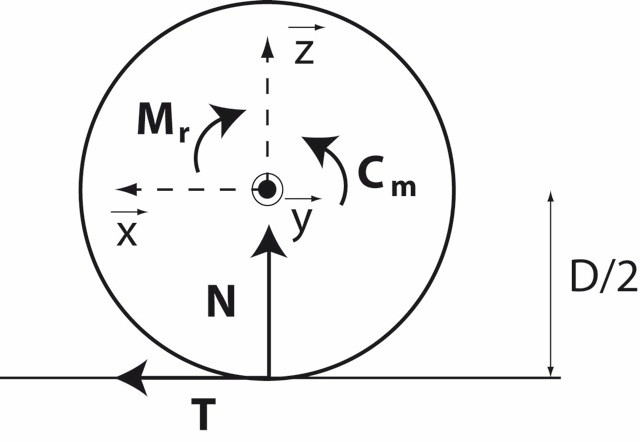
\includegraphics[width=.45\linewidth]{fig_16.png}
\caption{Schématisation des actions extérieures sur une roue\label{fig_16}}
\end{figure}
\fi

\question{Donner la relation entre le couple moteur $C_m$ et les autres actions extérieures.}
\ifprof
\begin{corrige}\textbf{ -- UPSTI}\\ 
On effectue le Bilan des Actions Mécaniques Extérieures Appliquées à la roue :
\begin{itemize}
\item Action de la plateforme sur la roue (liaison pivot d’axe $\vect{y}$;
\item Action du moteur $\vect{C_m}=C_m\vect{y}$;
\item Action résistante $\vect{M_r}=-kN\vect{y}$;
\item Action du sol sur la roue : $\vect{F_{\text{sol} \rightarrow \text{roue}}}$.
\end{itemize}

On applique le Théorème du Moment Statique au centre de la roue et on obtient :
$C_m - M_r - T\dfrac{D}{2} = 0$.

\end{corrige}
\else
\fi
\ifprof
\else
En lien avec l'évolution des efforts donnée dans l'Annexe 2, on trace sur la\autoref{fig_17} l'évolution
des couples $\indice{C}{m, AV}$, $\indice{C}{m,C}$ et $\indice{C}{m,AR}$ sur chaque paire de roues en fonction du temps lors du franchissement d'un obstacle de hauteur $H =\SI{400}{mm}$ et pour $\mu=2$.

\begin{figure}[H]
\centering
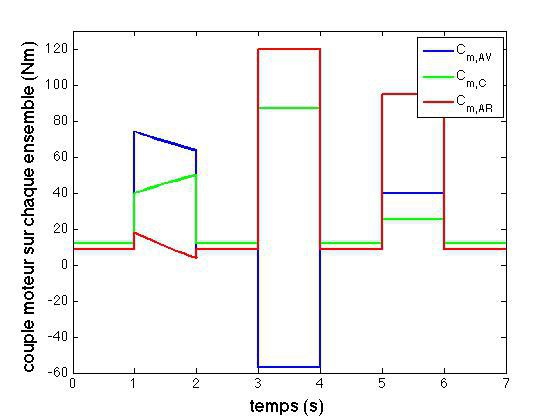
\includegraphics[width=.45\linewidth]{fig_17.png}
\caption{Evolution du couple sur chaque paire de roues\label{fig_17}}
\end{figure}
\fi


% Q3.12
\question{Conclure sur la valeur de couple à retenir pour le dimensionnement des moteurs, et
remettre en cause l'utilisation de l'hypothèse HYP2 pour ce dimensionnement.}
\ifprof
\begin{corrige}\textbf{ -- UPSTI}\\ 
Le couple maximal à retenir pour les moto-réducteurs est de \SI{120}{Nm}.
L’hypopthèse d’une valeur maximale (limite de glissement) pour la seule roue montant l’obstacle entraîne une surestimation de $C_m$. En réalité, il est possible que les trains avant et arrière soient plus ou moins chargés dans cette configuration.
\end{corrige}
\else
\fi

On cherche à présent la meilleure répartition du couple sur chaque roue, minimisant la puissance
motrice tout en évitant le glissement.

% Q3.13
\question{Proposer un algorithme de répartition du couple sur chaque roue, qui serait une alternative
à l'hypothèse HYP2 et permettrait de sélectionner des couples optimaux.}
\ifprof
\begin{corrige}\textbf{ -- UPSTI}\\ 
On peut par exemple calculer les couples résistants en prenant comme hypothèse un rapport $\dfrac{T}{N}$ constant sur les différents trains, ce qui aurait tendance à équilibrer la charge sur les différents trains.
Si l’on veut réellement limiter les couples moteurs, il faudrait faire la démarche inverse et atteindre la limite du glissement pour les roues les moins chargées.

\end{corrige}
\else
\fi


\subsection{Asservissement en couple – contrôle de traction}

\begin{obj}
Dans cette sous-partie, on étudie l’asservissement en couple des moteurs utilisé pour
limiter le glissement. Le cahier des charges à respecter est le suivant :

\begin{center}
\begin{tabular}{ll}
\hline
\textbf{Critère} & \textbf{Valeur} \\ \hline 
Dépassement autorisé & inférieur à 5 \% \\ 
Temps de réponse à 5 \% & inférieur à \SI{9}{ms} \\ \hline
\end{tabular}
\end{center}

\end{obj}
\ifprof
\else

La structure d’asservissement proposée est composée de deux correcteurs utilisés simultanément :
un correcteur de boucle de retour (nommé $C_{\text{fb}}( p)$) et un correcteur de boucle d'anticipation
(nommé $C_{\text{ff}}( p)$ ). L’étude menée ici concerne le comportement du système avec cette structure
de correction.
Le schéma d'asservissement est donné sur la \autoref{fig_18}.

\begin{figure}[H]
\centering
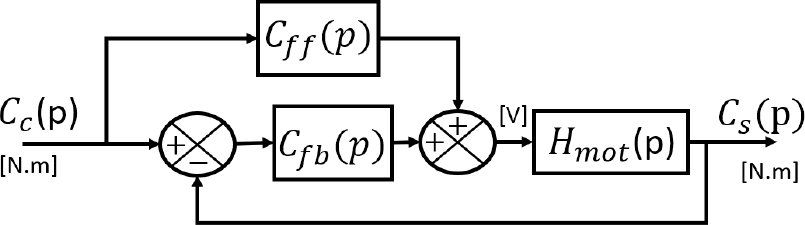
\includegraphics[width=.45\linewidth]{fig_18.png}
\caption{Schématisation de l'asservissement en couple \label{fig_18}}
\end{figure}


Le bloc  $\indice{H}{mot} (p)$ représente un moteur ayant pour fonction de transfert
$\indice{H}{mot} (p)=\dfrac{K_c}{K_c K_e+(R+Lp)( f +Jp)}$. Par identification, on trouve $\indice{H}{mot}= \dfrac{0,265}{0,4 p+200}$.

\fi

% Q3.14
\question{Énoncer, en justifiant, les hypothèses permettant de négliger les termes $L$ et $f$ pour
cette modélisation du moteur par une fonction de transfert du premier ordre.}
\ifprof
\begin{corrige}\textbf{ -- UPSTI}\\ 
Le modèle de connaissance est du second ordre. Or il nous est fourni un modèle du premier ordre. Cela signifie que le coefficient d’amortissement $\xi$ est supérieur à 1. Par conséquent la fonction de transfert du second ordre peut s’écrire comme un produit de 2 premiers ordres.
On a alors :
$\indice{H}{mot} (p)=\dfrac{K_c}{K_c K_e+Rf} \cdot \dfrac{1}{1+\dfrac{RJ+Lf}{K_c K_e+Rf}p+\dfrac{LJ}{K_c K_e+Rf}p^2}$ 
 
Si le coefficient de frottement est très faible (le couple dû aux frottements visqueux est très faible devant le couple électromagnétique), alors on peut considérer $f\simeq 0$
On a alors :
$\indice{H}{mot}(p)=\dfrac{1}{K_e} \dfrac{1}{1+\dfrac{RJ}{K_c K_e } p+\dfrac{LJ}{K_c K_e }p^2}$

L’inductance $L$ étant généralement faible (la tension aux bornes de l’inductance faible vis-à-vis des tensions électriques présentes dans le montage), on peut considérer $ L \simeq 0$.
Donc, on retrouve bien un modèle simplifié du 1er ordre tel que proposé.
 

\end{corrige}
\else
\fi

On néglige dans un premier temps la boucle d'anticipation ($\indice{C}{ff} =0$) et on prend
$\indice{C}{fb}( p)=\indice{K}{fb}+\dfrac{\indice{I}{fb}}{p}$.

% Q3.15
\question{Déterminer la fonction de transfert en boucle fermée.}
\ifprof
\begin{corrige}\textbf{ -- UPSTI}\\ 
$\indice{H}{mot} (p)=\dfrac{0,265}{0,4p+200}=\dfrac{\dfrac{0.265}{200}}{1+\dfrac{0.4}{200} p}=\dfrac{K}{1+\tau p}$

et $\dfrac{\indice{C}{S}(p)}{\indice{C}{C}(p)} $
$=\dfrac{\indice{C}{fb} (p) \indice{H}{mot} (p)}{1+\indice{C}{fb} (p) \indice{H}{mot} (p)}$
$=\dfrac{1+\dfrac{\indice{K}{fb}}{\indice{I}{fb}}  p}{1+\dfrac{K\indice{K}{fb}+1}{K\indice{I}{fb}} p+\dfrac{\tau}{K\indice{I}{fb} } p^2}$


\end{corrige}
\else
\fi

La \autoref{fig_19} représente l'évolution du dépassement et du temps de réponse à 5\% en fonction du
coefficient d'amortissement $\zeta$.

% Q3.16
\question{En s'aidant de la \autoref{fig_19}, exprimer les conditions sur les paramètres $\indice{K}{fb}$ et $\indice{I}{fb}$ permettant de respecter le cahier des charges.}
\ifprof
\begin{corrige}\textbf{ -- UPSTI}\\ 
Les paramètres du modèle élaboré en question précédente sont les suivants :
\begin{itemize}
\item  $\xi=\dfrac{1}{2} \dfrac{K\indice{K}{fb}+1}{K\indice{I}{fb}}\sqrt{\dfrac{K\indice{I}{fb}}{\tau}}$
\item  $\omega_0 = \sqrt{\dfrac{K\indice{I}{fb}}{\tau}}$.
\end{itemize}
Pour respecter le cahier des charges, il faut que $\xi \geq 0,7$ et $\omega_0 \geq \SI{333}{rad/s}$.


Les conditions traduites sur $\indice{I}{fb}$ et sur $\indice{K}{fb}$ donnent :

$\dfrac{K}{\tau} \omega_0^2 \leq \indice{I}{fb}$ soit $\indice{I}{fb}\geq 16,7\times 10^5$.

$\dfrac{\dfrac{2\xi \indice{I}{fb}}{\omega_0}-1}{K} > \indice{K}{fb}$
relation dont le résultat dépend de la valeur choisie pour $\indice{I}{fb}$.

\end{corrige}
\else
\fi

\ifprof\else
\begin{figure}[H]
\centering
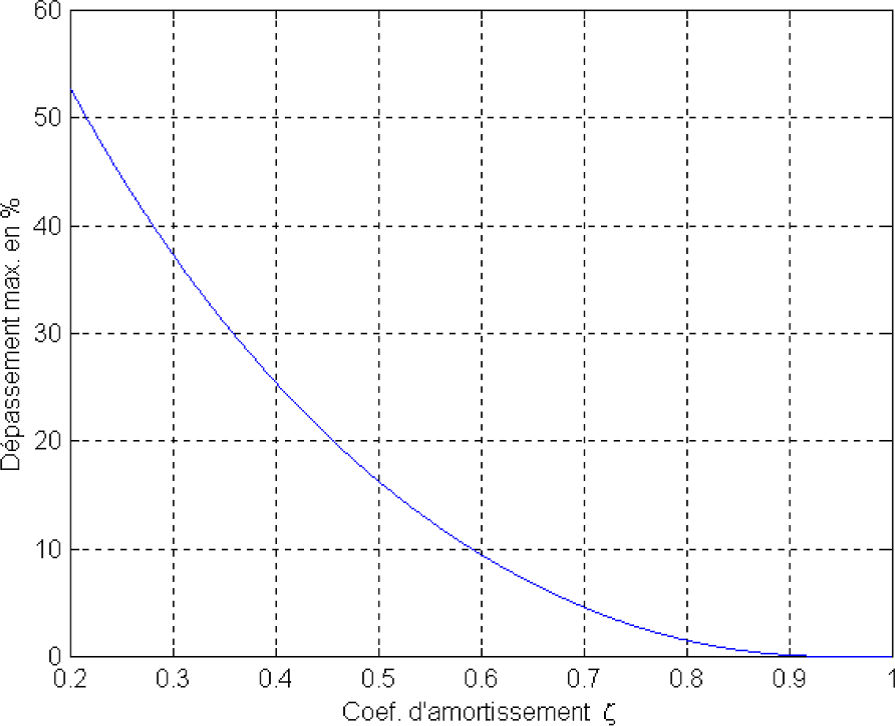
\includegraphics[width=.45\linewidth]{fig_19_a.png}
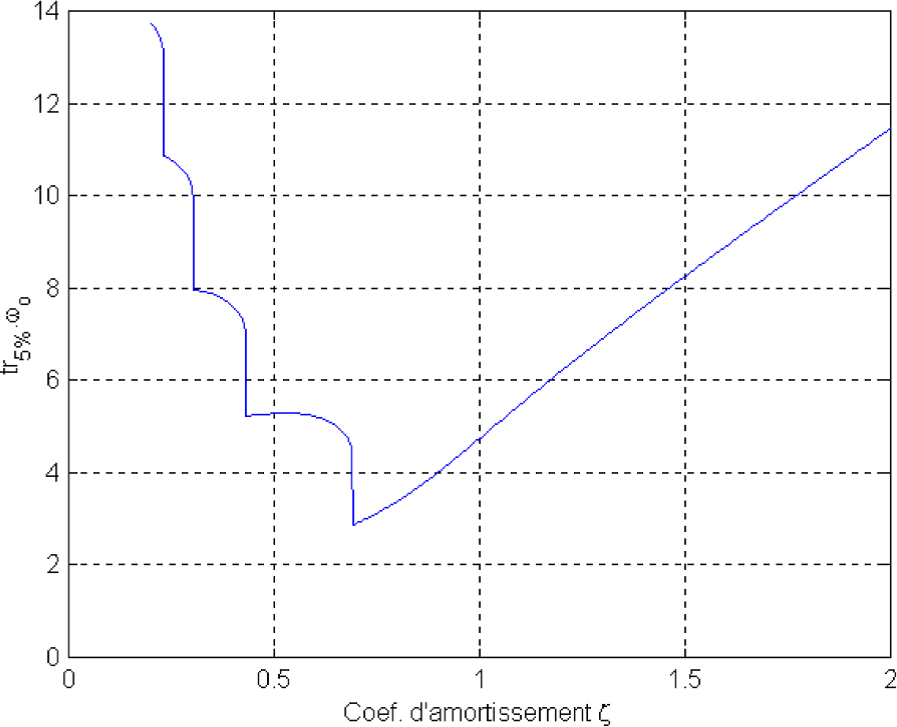
\includegraphics[width=.45\linewidth]{fig_19_b.png}
\caption{Dépassement et temps de réponse à 5\% en fonction de $\zeta$ \label{fig_19}}
\end{figure}


Par une technique d’optimisation, un bon jeu de paramètres trouvé est : $\indice{K}{fb}=30$ et $\indice{I}{fb}=200\times10^{3}$.
\fi

% Q3.17
\question{Calculer la valeur du dépassement et le temps de réponse.}
\ifprof
\begin{corrige}\textbf{ -- UPSTI}\\ 
Dans le cas avec le jeu de paramètre correct, on a : $\omega_0 \simeq \SI{365}{rad/s}$, $\xi \simeq 0,701$.

Donc, d’après les courbes on trouve : $t_{R5\%} = \SI{8}{ms}$.


\end{corrige}
\else
\fi

% Q3.18
\question{Tracer %sur le document réponse DR2 
le diagramme de Bode asymptotique de la fonction de transfert en boucle ouverte. Discuter des marges de gain et de phase.}
\ifprof
\begin{corrige}\textbf{ -- UPSTI}\\ 
La fonction de transfert en Boucle Ouverte s’exprime ainsi :
$\text{FTBO}(p)=\indice{C}{fb} (p) \indice{H}{mot} (p)=\left(30+\dfrac{200\times 10^3}{p}\right)
\dfrac{0,265}{0,4p+200}=265\left(1+\dfrac{p}{6667}\right)\dfrac{1}{1+p/500}$.

\begin{figure}[H]
\centering
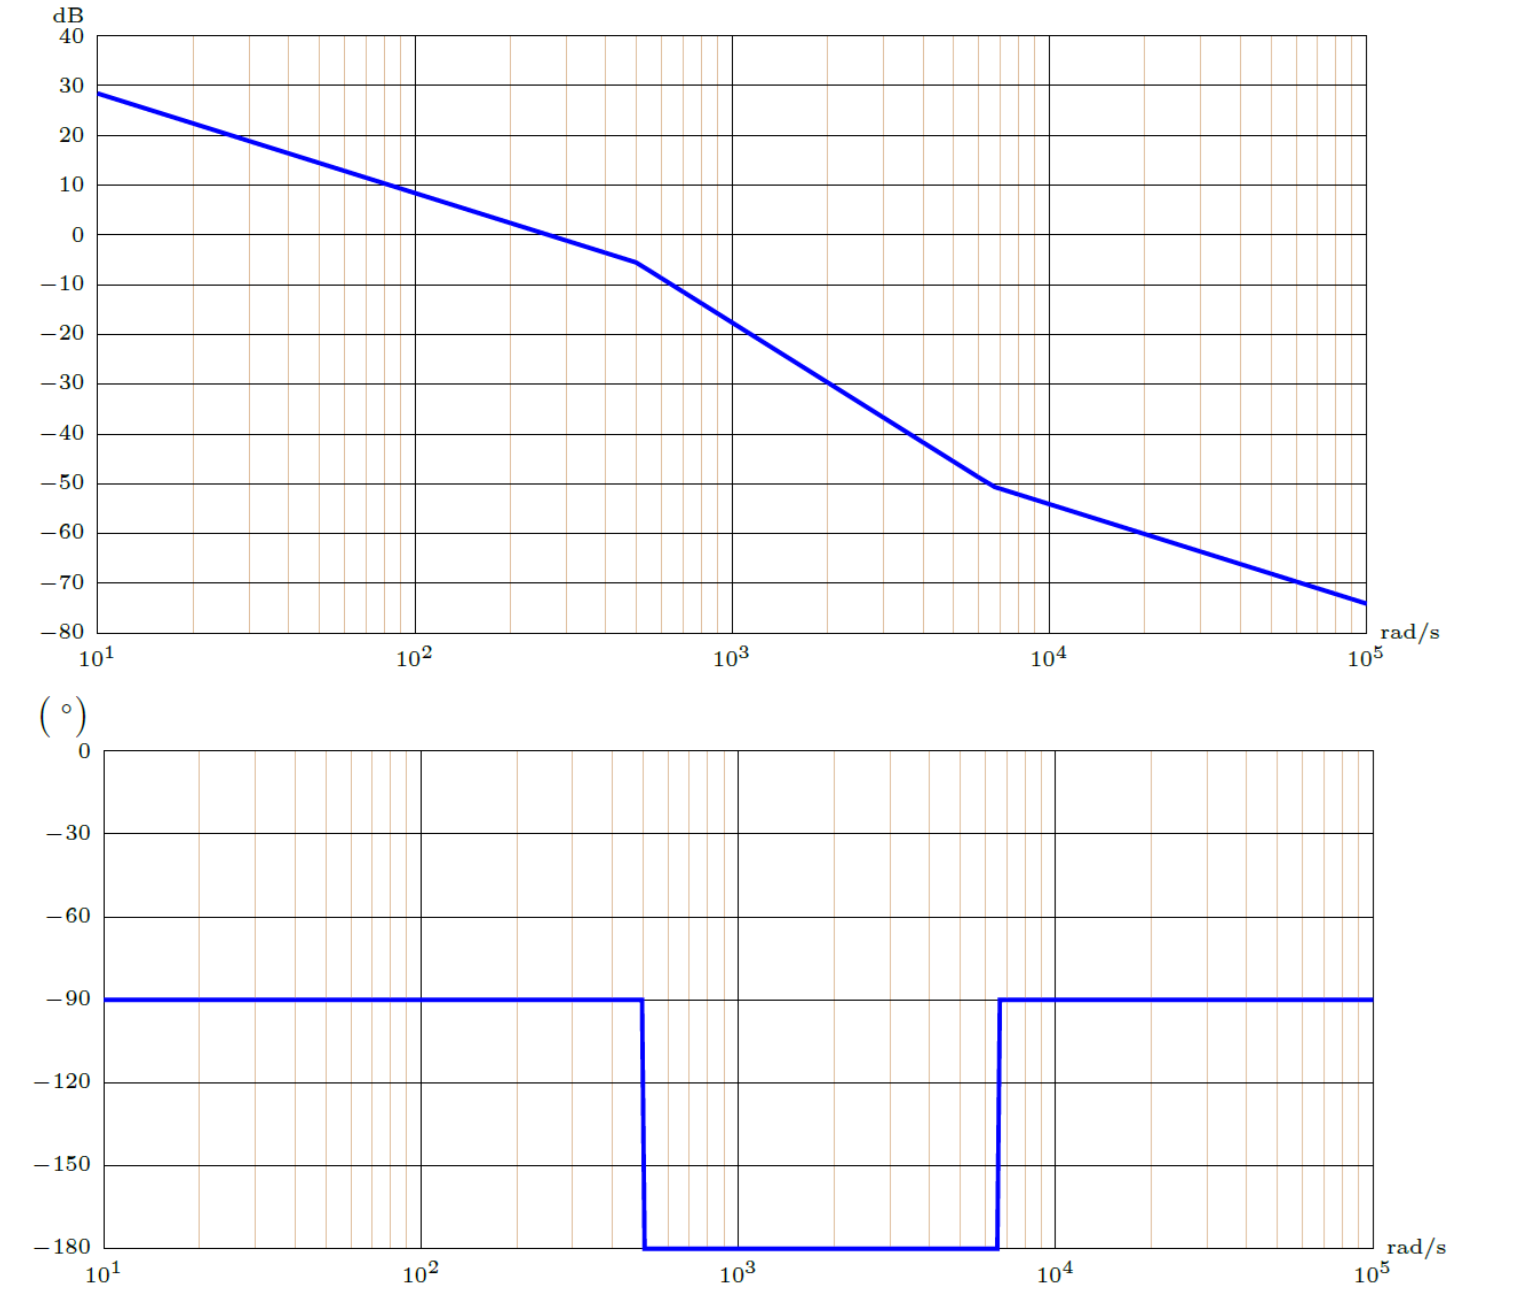
\includegraphics[width=.85\linewidth]{cor_Q318.png}
\end{figure}

La marge de gain est infinie (ou non définie) car la phase n’atteint jamais $-180\degres$.

La marge de phase est nécessairement positive, car la phase est strictement supérieure à $-180\degres$. Donc le système est bien stable en boucle fermée.


\end{corrige}
\else
\fi


On considère à présent la structure d'asservissement complète, avec le correcteur $\indice{C}{ff} (p)$.

% Q3.19
\question{Exprimer la fonction de transfert en boucle fermée du système en fonction de $\indice{H}{mot}( p)$, $\indice{C}{fb} (p)$ et $\indice{C}{ff} (p)$.}
\ifprof
\begin{corrige}\textbf{ -- UPSTI}\\ 
$\dfrac{C_S (p)}{C_C (p)}=\left(
1+\dfrac{\indice{C}{ff} (p)}{\indice{C}{fb} (p)}\right)
\dfrac{\indice{H}{mot}(p) \indice{C}{fb}(p)}{1+\indice{H}{mot}(p) \indice{C}{fb}(p)}$

\end{corrige}
\else
\fi

% Q3.20
\question{Que se passe-t-il si le correcteur vaut $\indice{C}{ff} (p)= \dfrac{1}{\indice{H}{mot} (p)}$ ? Quel est l’intérêt et le risque ?}
\ifprof
\begin{corrige}\textbf{ -- UPSTI}\\ 
En admettant que l’on puisse réaliser un tel système (en fait, le système étant composé d’un gain et d’un dérivateur pur, il faudrait rajouter du filtrage afin d’avoir un système causal), on obtient après simplification :
 
$\dfrac{C_S (p)}{C_C (p)}=\left(
1+\dfrac{\indice{C}{ff} (p)}{\indice{C}{fb} (p)}\right)
\dfrac{\indice{H}{mot}(p) \indice{C}{fb}(p)}{1+\indice{H}{mot}(p) \indice{C}{fb}(p)}=1$


L’intérêt théorique d’un tel système est donc évident puisqu’il s’agit d’un système dont la réponse correspond parfaitement à la consigne.
Cependant, pour y parvenir, il faut parfaitement maîtriser les paramètres du modèle du moteur $\indice{H}{mot} (p)$.

Un risque est donc de ne pas avoir un modèle suffisamment précis de $\indice{H}{mot} (p)$ et donc d’avoir des réactions imprévisibles et non désirées du correcteur.

Un autre  écart entre la théorie et la réalisation pratique du correcteur  est lié à la saturation de la commande. Un tracé de la réponse du système à un échelon de commande réalisé avec le correcteur théorique (modèle fourni dans ce dossier) montre la commande théorique du système.

\end{corrige}
\else
\fi

Pour une fonction de transfert $\indice{C}{fb} (p)$ fixée, on considère le correcteur $\indice{C}{ff}(p)$ comme un gain
proportionnel variable. Les courbes de réponse pour différentes valeurs de ce gain proportionnel
sont données dans l'Annexe 3.

% Q3.21
\question{Quelles conclusions peut-on en tirer sur l'effet du correcteur $\indice{C}{ff} (p)$?}
\ifprof
\begin{corrige}\textbf{ -- UPSTI}\\ 
Ce correcteur à tendance à améliorer la rapidité sans trop dégrader la stabilité. Les critères de rapidité (temps de réponse à 5\%) et de stabilité (dépassement autorisé) sont respectés, voire même améliorés pour $\indice{C}{ff}  = 100$.
\end{corrige}
\else
\fi


\section{Étude de l'action de préhension \label{sec_5}}

\begin{obj}
L'objectif de cette partie est de valider les performances de serrage de la pince et de vérifier
les critères suivants du cahier des charges.
\begin{center}
\begin{tabular}{ll}
\hline
\textbf{Critère} & \textbf{Valeur} \\ \hline \hline
Diamètre des objets à saisir entre & \SI{40}{mm} et \SI{300}{mm} \\ \hline
Masse maximale des objets à saisir & \SI{2,5}{kg} \\
\hline
\end{tabular}
\end{center}
\end{obj}


\subsection{Actions mécaniques dans la pince}

\begin{obj}
Dans cette sous-partie, on établit la transmission des actions mécaniques entre
l'actionneur et l'effecteur et on quantifie les actions à fournir par l'actionneur pour respecter
le cahier des charges.
\end{obj}


La pince de préhension, servant à collecter les échantillons de roche ou à poser/prendre des
instruments sur le sol, est une pince à trois doigts (préhenseur tridigital, voir \autoref{fig_23}). Par
symétrie, on restreint l'étude à un seul doigt.
La chaîne cinématique correspondante est schématisée (modélisation plane) sur la \autoref{fig_23} ; elle
est constituée :
\begin{itemize}
\item du bâti 0 lié au bras manipulateur du système ROBOVOLC, auquel on associe le repère $\left(P,\vect{x_P},\vect{y_P},\vect{z_P}\right)$ avec
$\vect{x_P}$ la verticale descendante ;
\item  d'un vérin 1 en liaison glissière de direction $\vect{x_P}$ avec le bâti 0 ;
\item  d'une tige 2 en liaison pivot d'axe $\left(H,\vect{z_P}\right)$ avec le vérin 1 ;
\item  de deux biellettes 3 et 4 parallèles et en liaisons pivot d'axes respectifs $\left(A,\vect{z_P}\right)$ et $\left(C,\vect{z_P}\right)$
avec le bâti 0. La biellette 3 est également en liaison pivot d'axe $\left(E,\vect{z_P}\right)$ avec la tige 2 ;
\item  d'un mors 5 en liaisons pivot d'axes $\left(B,\vect{z_P}\right)$ et $\left(D,\vect{z_P}\right)$ avec les biellettes 3 et 4 ;
\item  d'un galet 6 en liaison rotule de centre $Q$ avec le mors 5 et en contact avec l'objet à saisir.
\end{itemize}
Les points $A$ , $B$ , $C$ , $D$ forment un parallélogramme. On introduit le paramétrage suivant :
$d=\vect{HP} \cdot \vect{y_P}=\vect{AP} \cdot \vect{y_P}=\vect{CP} \cdot \vect{y_P}$, 
$CE = EH = \ell_2$, 
$AC = BD = \ell_3$,
$AB = CD = \ell_4$,
$\vect{DQ} = L_5\vect{x_P} + \ell_5 \vect{y_P}$, 
$\vect{QS} = \ell_6\vect{y_P}$
ainsi que les angles
$\alpha = \left(\vect{HC},\vect{HE}\right)$
et  $\beta = \left(\vect{y_P},\vect{EC}\right)$.

On donne $d = \SI{50}{mm}$, $\ell_2 =\SI{100}{mm}$, $\ell_4 =\SI{150}{mm}$, $\ell_5 =\SI{20}{mm}$, $\ell_6 =\SI{15}{mm}$.

\begin{figure}[H]
\centering
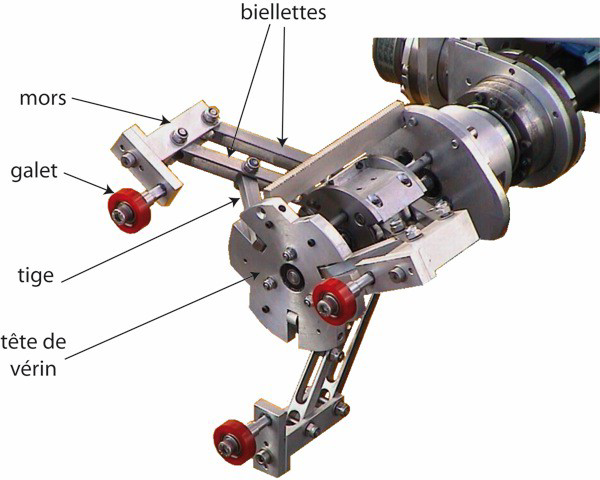
\includegraphics[width=.45\linewidth]{fig_23a.png}
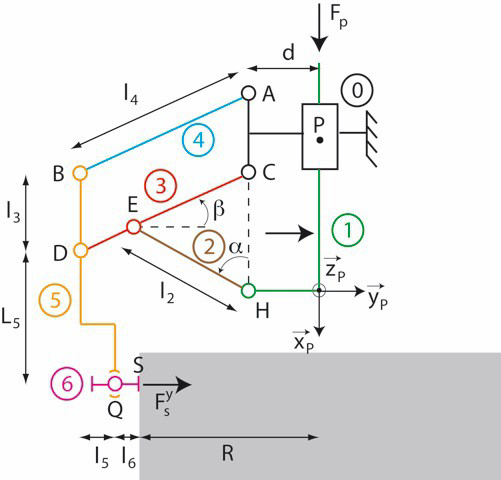
\includegraphics[width=.45\linewidth]{fig_23b.png}
\caption{Pince utilisée sur le système ROBOVOLC et schéma cinématique associé \label{fig_23}}
\end{figure}


Le contact entre le galet 6 et l'objet est modélisé par une liaison linéaire rectiligne d'axe $\left(S,\vect{x_P}\right)$ et
de normale $\vect{y_P}$ .
Dans une première approche, on considère que toutes les liaisons sont parfaites. De plus, le poids
des pièces composant la pince est négligé.
L'objet à saisir est modélisé par un cylindre à base circulaire de rayon $R$.


% Q5.1
\question{Donner le lien entre les angles $\alpha$ et $\beta$, ainsi que l'expression de ces angles en fonction du
rayon $R$ de l'objet et des données géométriques.}
\ifprof
\begin{corrige}
Une fermeture géométrique angulaire dans le triangle $CEH$ donne immédiatement :  $\alpha + \beta =\dfrac{\pi}{2}$.

Une fermeture géométrique linéaire permet de déterminer la relation entre  $\alpha$ (ou $\beta$), $R$ et les dimensions du mécanisme.
On trouve (en projetant sur l’axe $\vect{x}$) :
$\left\{
\begin{array}{l}
R = d + l_4 \cos\beta -l_5 - l_6 \\
R = d + l_4 \sin\beta -l_5 - l_6 \\
\end{array}
\right.
$.

\end{corrige}
\else
\fi

% Q5.2
\question{Montrer que la liaison équivalente entre le mors 5 et l'objet à saisir est une liaison ponctulle de normale $\left(S,\vect{y_P}\right)$. Cette liaison équivalente
sera utilisée dans la suite de cette partie.}
\ifprof
\begin{corrige}
Les liaisons étant en série, il est plus direct de passer par les torseurs cinématiques. Nous avons ici l’association d’une liaison rotule et d’une liaison appui plan en série
$\torseurcin{V}{5}{\text{objet}} = \torseurcin{V}{5}{6} + \torseurcin{V}{6}{\text{objet}}$.

$\torseurcin{V}{5}{\text{objet}} 
= 
\torseurl{\omega_{x56} \vect{x_P}+\omega_{y56} \vect{y_P}+\omega_{z56} \vect{z_P}}
{\vect{0}}{Q}
+ \torseurl{\omega_{y60} \vect{y_P}}{V_x \vect{x_P}+V_z \vect{z_P}}{Q}
= 
\torseurl{\omega_{x} \vect{x_P}+\omega_{y} \vect{y_P}+\omega_{z} \vect{z_P}}
{V_x \vect{x_P}+V_z \vect{z_P}}{Q}
$.

Il s’agit du torseur d’une liaison ponctuelle de normale $(Q,\vect{y_P})$,  la forme du torseur est maintenue sur la droite $(Q,\vect{y_P})$, la liaison peut donc s’exprimer également comme une ponctuelle de normale  $(S,\vect{y_P})$.

\end{corrige}
\else
\fi

% Q5.3
%\question{Calculer l'hyperstatisme du modèle plan du mécanisme global de la pince (\autoref{fig_23}).}

% Q5.4
\question{Donner l'orientation de l'effort dans les liaisons pivot situées en $B$ et en $E$.}
\ifprof
\begin{corrige}
Les solides 2 et 4 sont soumis chacun à 2 glisseurs, par conséquent, les directions des efforts  en $B$ et $E$ sont respectivement $\vect{AB}$ et $\vect{EH}$.
\end{corrige}
\else
\fi


L'ouverture/fermeture de la pince est réalisée par un moteur électrique et un système vis-écrou
fournissant un effort de poussée $\vect{F_P}=F_p\vect{x_P}$ sur le vérin 1 en amont de la pince. D'autre part, on
introduit à présent un modèle de frottement au contact entre le galet 6 et l'objet à saisir. Ce modèle
se traduit au niveau de la liaison équivalente entre le mors 5 et l'objet à saisir par un torseur
statique de la forme : $\torseurstat{T}{5}{\text{objet}}=\torseurl{-F_S^x\vect{x_P}+F_S^y\vect{y_P}}{\vect{0}}{S}$ 
où $F_S^x$ est l'effort tangentiel et $F_S^y$ est l'effort normal (ou de serrage) au contact.

% Q5.5
\question{Par une étude statique, montrer que les efforts $F_P$, $F_S^x$ et $F_S^y$ 
y sont liés par la relation $F_P = K \left( \tan \beta F_S^y - F_S^x\right)$  
où l'expression de la constante $K$ est à préciser en fonction de $\ell_2$ et $\ell_4$.
Montrer également que cette relation est indépendante de la longueur $L_5$ et expliquer l'avantage technique de ce résultat. }
\ifprof
\begin{corrige}~\\
\begin{figure}[H]
\centering
{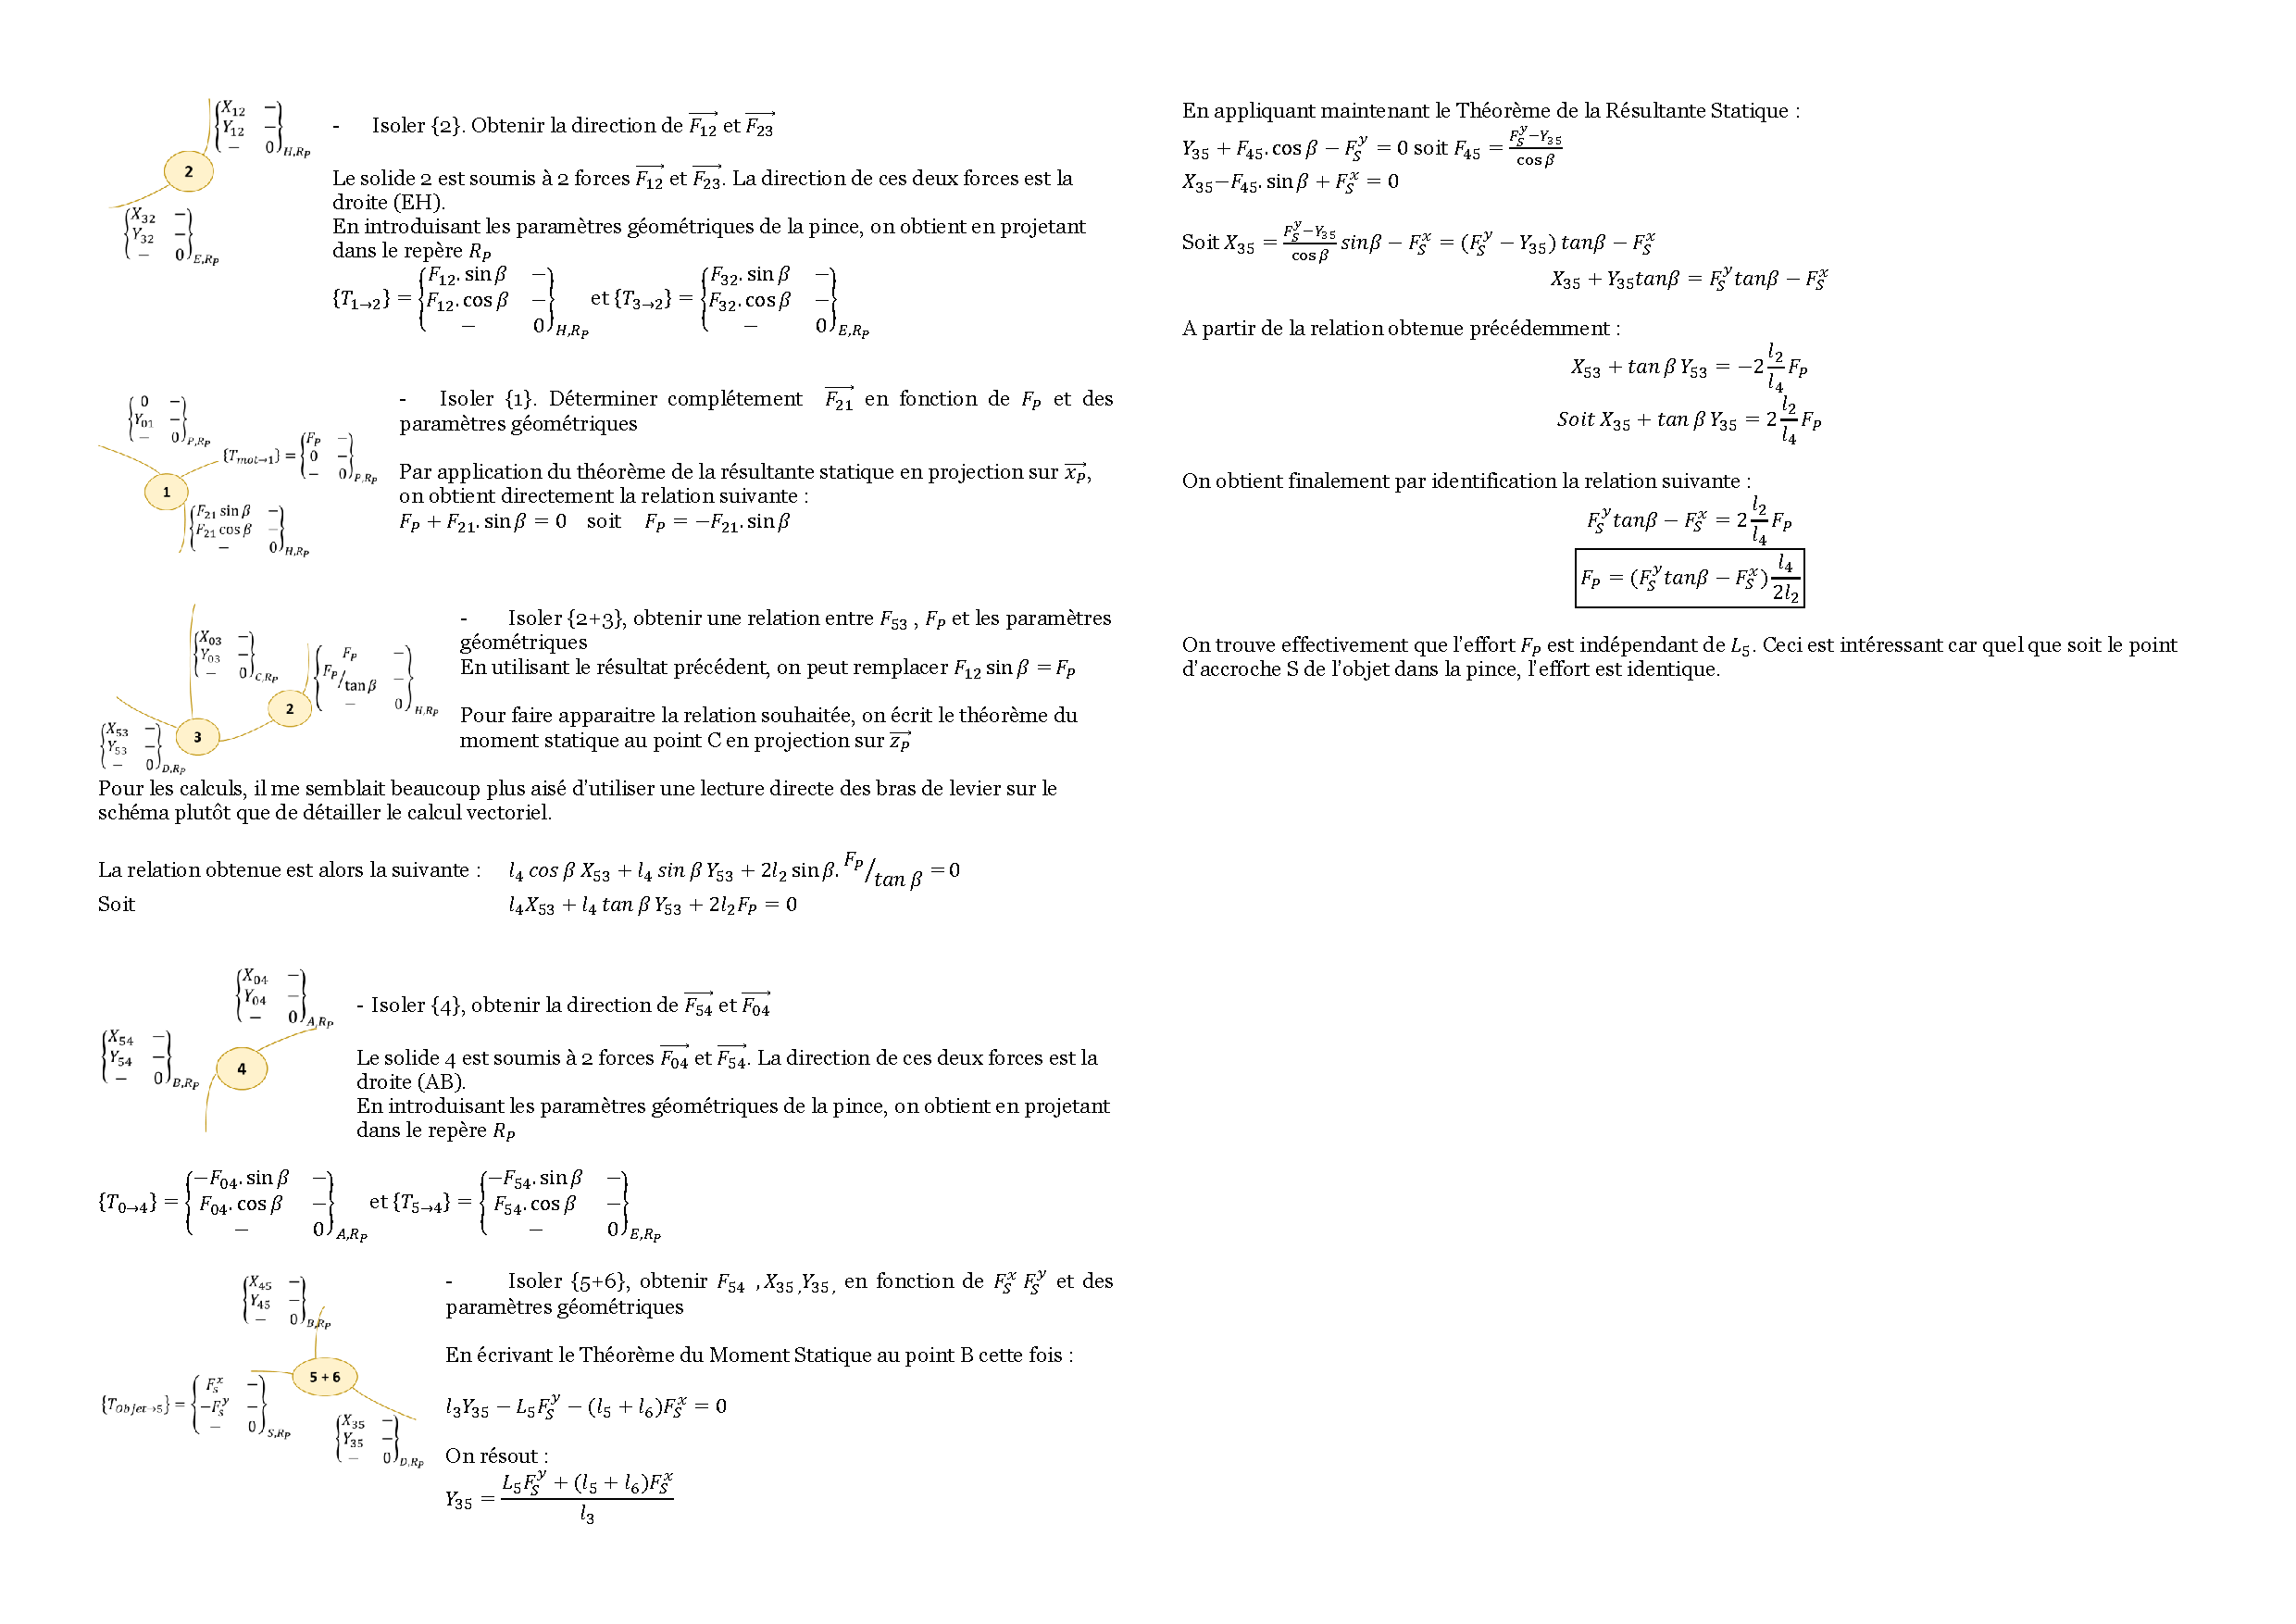
\includegraphics[width=\linewidth]{PFS}}
\end{figure}

\end{corrige}
\else
\fi

On représente sur la \autoref{fig_24}  l'évolution de $\tan \beta$ en fonction du rayon $R$ de l'objet à saisir sur la plage $R =[\SI{20}{mm}, \SI{165}{mm}]$.

\begin{figure}[H]
\centering
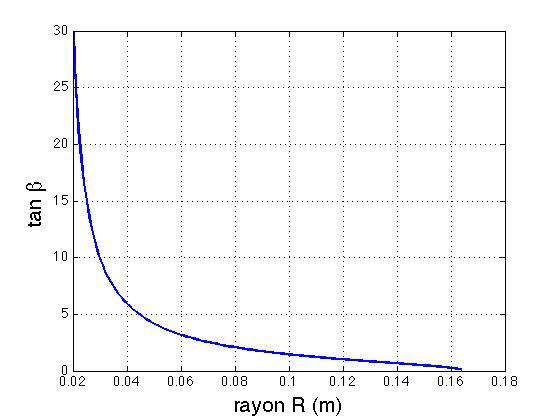
\includegraphics[width=10cm]{fig_24.png}
\caption{Evolution de $\tan \beta$ en fonction de $R$ \label{fig_24}}
\end{figure}


%Q5.6 : 
\question{Commenter ce graphe, en particulier pour les valeurs extrêmes du rayon $R$.}
\ifprof
\begin{corrige}
On remarque que :
\begin{itemize}
\item quand $R$ est grand, l’effort $F_P$est quasi-indépendant de l’effort normal $F_S^y$ de la pince sur l’objet. 
\item quand $R$ est petit, l’effort $F_P$ dépend quasi-uniquement de l’effort normal $F_S^y$. La capacité de préhension est fortement diminuée pour des petits rayons.
\end{itemize}
\end{corrige}
\else
\fi

%Q5.7 : 
\question{En supposant un modèle de frottement de Coulomb (le coefficient de frottement est noté $f$), 
montrer que l'objet peut être saisi et soulevé sans aucune action de poussée $F_p$ du moteur
lorsque le rayon de l'objet est tel que $R \geq R_{\text{min}}$. On précisera l'expression de $ R_{\text{min}}$ , on donnera sa
valeur pour $f =2$, et on commentera ce caractère particulier de la pince en donnant un avantage
et un inconvénient.}
\ifprof
\begin{corrige}
En supposant un modèle de frottement de Coulomb, on a à la limite de l'adhérence (action de l’objet 6 sur le cône de frottement)
$|F_S^x |=f |F_S^y |$. L’effort $F_P$ est nul lorsque $\tan\beta =f$.
Dans ces conditions, le rayon 
$
R=R_{\text{min}} = d+l_4 \sin \left (\tan^{-1} f \right) -l_5 -l_6$.

\end{corrige}
\else
\fi

%Q5.8 : 
\question{Pour $R < R_{\text{min}}$, donner la relation entre l'effort de poussée $F_p$ et la masse $m_{\text{objet}}$ de l'objet
à saisir, ainsi qu'entre l'effort de poussée $F_p$ et l'effort de serrage$F_S^y$ . En déduire la valeur de
l'effort de poussée maximal à fournir pour respecter le cahier des charges avec $f =2$.}
\ifprof
\begin{corrige}
Dans le cas où $R<R_{\text{min}}$ on a :
$F_P=\left(\dfrac{m_{\text{objet}}g}{3} \tan \beta -f \dfrac{m_{\text{objet}} g}{3}\right) \dfrac{l_4}{2l_2}$ 

Le cahier des charges impose  $R_{\text{min}}=0,04$ soit  $\tan\beta =6$ d’après la figure 24 et  $m_{\text{maxi}}=\SI{2,5}{kg}$

Dans ces conditions,
$F_P=\left(\dfrac{2,5\times 10}{3} \times 6- \dfrac{2 \times 2,5\times 10}{3}\right)  \dfrac{3}{4}=\SI{25}{N}$.

Pour les trois doigts, l’effort sera donc de \SI{75}{N}.

\end{corrige}
\else
\fi

\subsection{Asservissement de l'effort}

\begin{obj}
Dans cette sous-partie, on étudie l’asservissement en effort de la pince. En lien avec la
sous-partie précédente, on se place dans la configuration $R < R_{\text{min}}$ et on donne la relation
$F_s^y = K_{\beta} F_p$.
\end{obj}


La pince a un capteur d'effort pour mesurer et contrôler la force de serrage. Pour l'asservissement
de la pince, une régulation en effort est faite. Le schéma blocs de la \autoref{fig_25} présente la structure
de contrôle de la pince.


\begin{figure}[H]
\centering
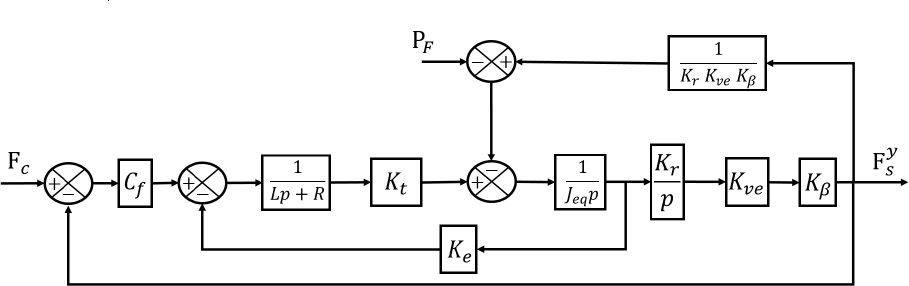
\includegraphics[width=.9\linewidth]{fig_25.png}
\caption{Schéma d'asservissement \label{fig_25}}
\end{figure}


%Q5.9 : 
\question{Quel est l'intérêt pratique de la régulation mise en place ?}
\ifprof
\begin{corrige}
La régulation en place permet de contrôler l’effort normal et donc de contrôler le non-glissement de l’objet par rapport à la pince.
\end{corrige}
\else
\fi
Pour l’étude en asservissement de la pince, on fixe $K_{\beta} = 2,2$.
On donne les caractéristiques du système suivantes.

\begin{table}[H]
\centering
\begin{tabular}{lll}
\hline
$R$ &  résistance d'induit 		& $\SI{7,2}{\Omega}$ \\ \hline
$L$ &   inductance d'induit 	& \SI{2,56}{mH} \\ \hline
$K_t$ &  constante de couple 	& \SI{0,82}{Nm/A} \\ \hline
$K_e$ &  constante de fcem 	& \SI{86}{V/1000tr/min} \\ \hline
$J_{\text{eq}}$ &  moment d'inertie 	& \SI{3,45e-4}{ kg m^2} \\ \hline
$Kr$ &  rapport du réducteur 	& $54/33=1,636$ \\ \hline
$K_{\text{ve}}$ & pas du système vis-écrou & $\SI{4}{mm}$  \\ \hline
\end{tabular}
\end{table}


%Q5.10 : 
\question{En considérant $P_F=0$ (perturbation nulle) et $L=0$ (inductance nulle), calculer la fonction de transfert
$\dfrac{F_S^y}{F_c}$ et la mettre sous la forme canonique $\dfrac{K}{1+Ap+Bp^2}$. Identifier les paramètres $K$,
$A$ et $B$.}
\ifprof
\begin{corrige}

$\dfrac{F_S^y (p)}{F_C (p)}=\dfrac{C_f K_t K_r K_{ve} K_{\beta}}{R+C_f K_t K_r K_{ve} K_{\beta} } \times \dfrac{1}{1+\dfrac{K_e K_t}{R+C_f K_t K_r K_{ve} K_{\beta} }p+\dfrac{RJ_{eq}}{R+C_f K_t K_r K_{ve} K_{\beta} } p^2}$.


Par identification, on obtient :
$K=\dfrac{C_f K_t K_r K_{ve} K_{\beta}}{R+C_f K_t K_r K_{ve} K_{\beta}}$
$A=\dfrac{K_e K_t}{R+C_f K_t K_r K_{ve} K_{\beta} }$;
$B=\dfrac{RJ_{\text{eq}}}{R+C_f K_t K_r K_ve K_{\beta} }$.

\end{corrige}
\else
\fi

On souhaite une erreur de position inférieure à 1\%.

%Q5.11 : 
\question{Calculer la valeur de $C_f$ permettant de respecter cette contrainte.}
\ifprof
\begin{corrige}
L’erreur statique $\varepsilon_p$ pour une entrée en échelon d’amplitude $F_{\text{c0}}$ vaut :

$\varepsilon_p=(1-K) F_{\text{c0}}=\dfrac{R}{R+C_f K_t K_r K_{ve} K_{\beta} } F_{\text{c0}}$.

Pour obtenir une erreur inférieure à 1\%, il faut :
$C_f>\dfrac{0,99R}{0,01K_t K_r K_{ve} K_{\beta} } \simeq 60370$.

\end{corrige}
\else
\fi

%Q5.12: 
\question{Bien qu’il y ait un intégrateur dans la chaîne directe, indiquer pourquoi l’erreur statique est non-nulle.}
\ifprof
\begin{corrige}
L’intégrateur est placé  après la perturbation (modélisée comme un couple résistant sur le moteur). L’erreur ne peut donc être nulle malgré la présence de l’intégrateur (il y a une perturbation inhérente à l’effort $F_S^y$).
On peut aussi dire que la FTBO est de classe 0 (on ne retrouve pas l’intégrateur pur dans l’écriture de la FTBO).

\end{corrige}
\else
\fi

%Q5.13: 
\question{En considérant une valeur du correcteur permettant de valider le critère d’erreur de
position, ce critère sera-t-il toujours validé si on ne néglige plus les perturbations ? Comment le
démontrer ?}
\ifprof
\begin{corrige}
La perturbation agissant sur la valeur de l’erreur globale, en l’absence d’intégrateur pur en amont de la perturbation, le critère ne sera plus systématiquement validé. On peut le démontrer par le Théorème de la valeur Finale par exemple.
\end{corrige}
\else
\fi

%Q5.14: 
\question{Le coefficient  $K_{\beta}$ a-t-il une influence sur l’asservissement ? Pourquoi ne peut-on pas
considérer $K_{\beta}$ comme une constante ?}
\ifprof
\begin{corrige}
Le coefficient $K_{\beta}$ représente la loi entrée-sortie du mécanisme reliant la position linéaire du vérin et la position de la pince. Cette relation est non-linéaire car elle fait intervenir des fonctions trigonométriques de l’angle ${\beta}$. Bien évidemment, ce coefficient a une influence sur le comportement de l’asservissement et un choix sera fait sur la zone de fonctionnement qui sera linéarisée.
\end{corrige}
\else
\fi

Pour des raisons techniques, il n'est pas possible d'utiliser un capteur d'effort en bout de pince.

%Q5.15 : 
\question{Est-il techniquement possible d'asservir le système sans ce capteur d'effort ? Expliquer le
raisonnement.}
\ifprof
\begin{corrige}
Bien qu’il ne soit pas possible de positionner un capteur d’effort, il est possible d’asservir cette grandeur. En effet, il est possible de trouver une grandeur image de l’effort normal par le biais par exemple de la mesure du courant électrique circulant dans l’induit du moteur. Ce courant est une image du couple moteur qui sera lui-même image de l’effort normal. Dans ce contexte, la relation non-linéaire du mécanisme sera une difficulté supplémentaire à surmonter si la mesure est indirecte.
\end{corrige}
\else
\fi

Dans l'étude précédente, la masse de l'objet et le coefficient de frottement entre la pince et l'objet
sont supposés connus. Cependant, ce n’est pas le cas en pratique et il peut en résulter un
glissement possible de l’objet si ces paramètres sont mal évalués.

%Q5.16 : 
\question{Quel moyen peut-on imaginer afin de limiter le glissement de l’objet ? Expliquer le
raisonnement.}
\ifprof
\begin{corrige}
Afin de limiter le glissement, il faut :
\begin{itemize}
\item augmenter l’effort normal (et maitriser également le rayon de la pièce soulevée);
\item jouer sur le couple de matériaux en contact afin de maximiser le coefficient d’adhérence.
\end{itemize}

\end{corrige}
\else
\fi



\section*{Annexe 1 -- Diagrammes SYSML}

\begin{center}
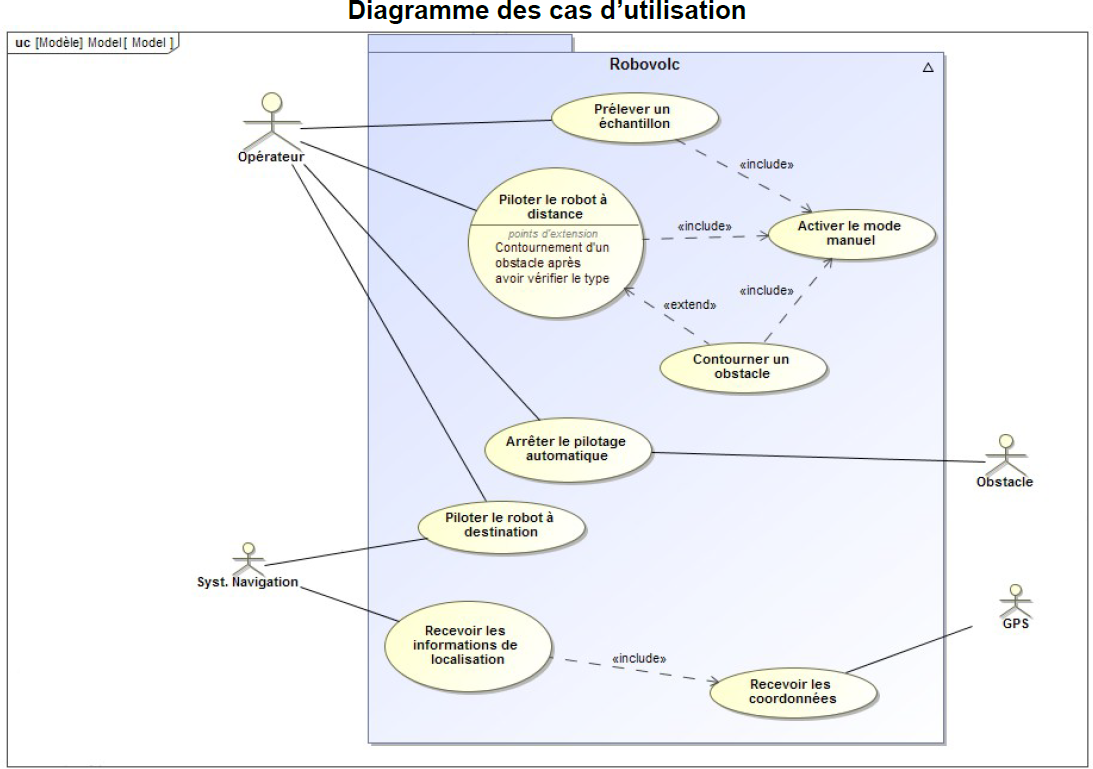
\includegraphics[width=.9\linewidth]{ann_01.png}

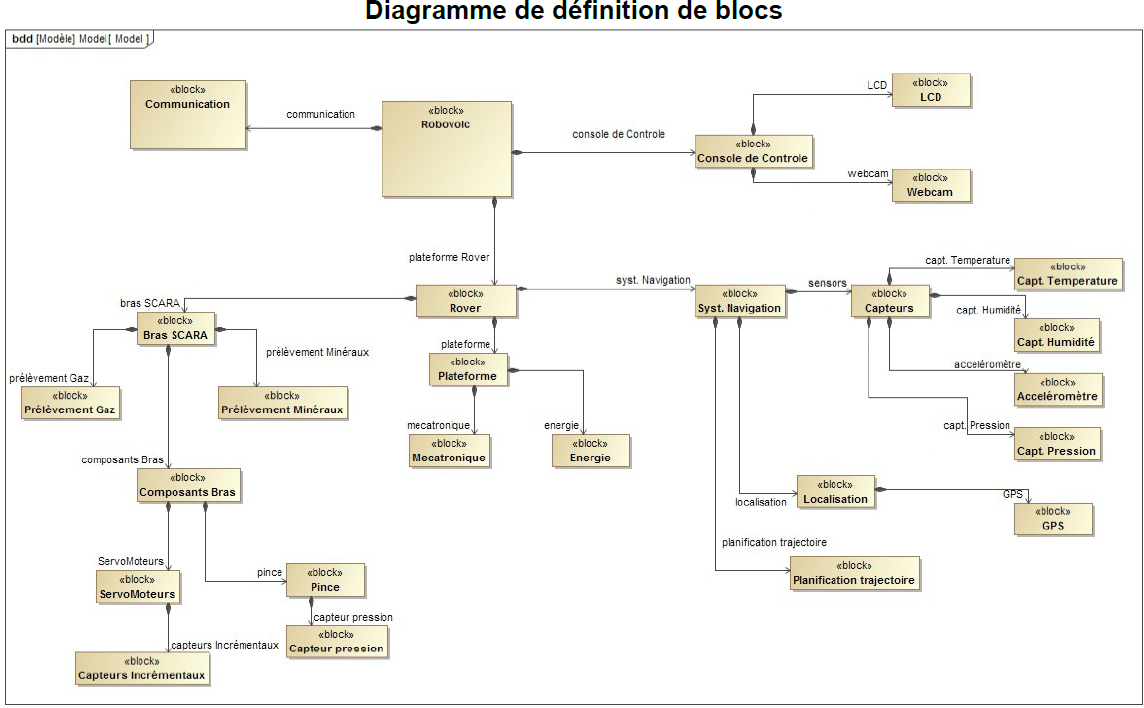
\includegraphics[width=.9\linewidth]{ann_02.png}
\end{center}

\section*{Annexe 2 -- Évolution simulée des efforts sur les roues}

\begin{center}
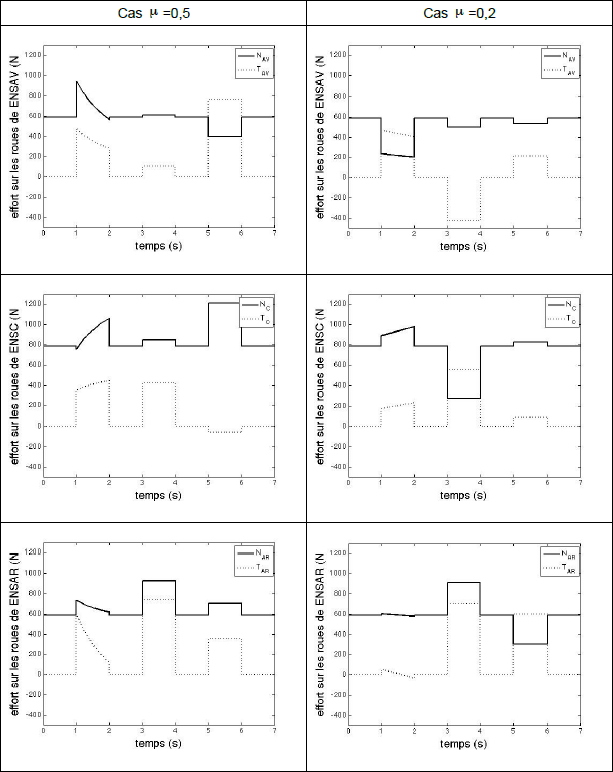
\includegraphics[width=.95\linewidth]{ann_02_.png}
\end{center}


\section*{Annexe 3 -- Évolution simulée de la réponse de l'asservissement}

\begin{center}
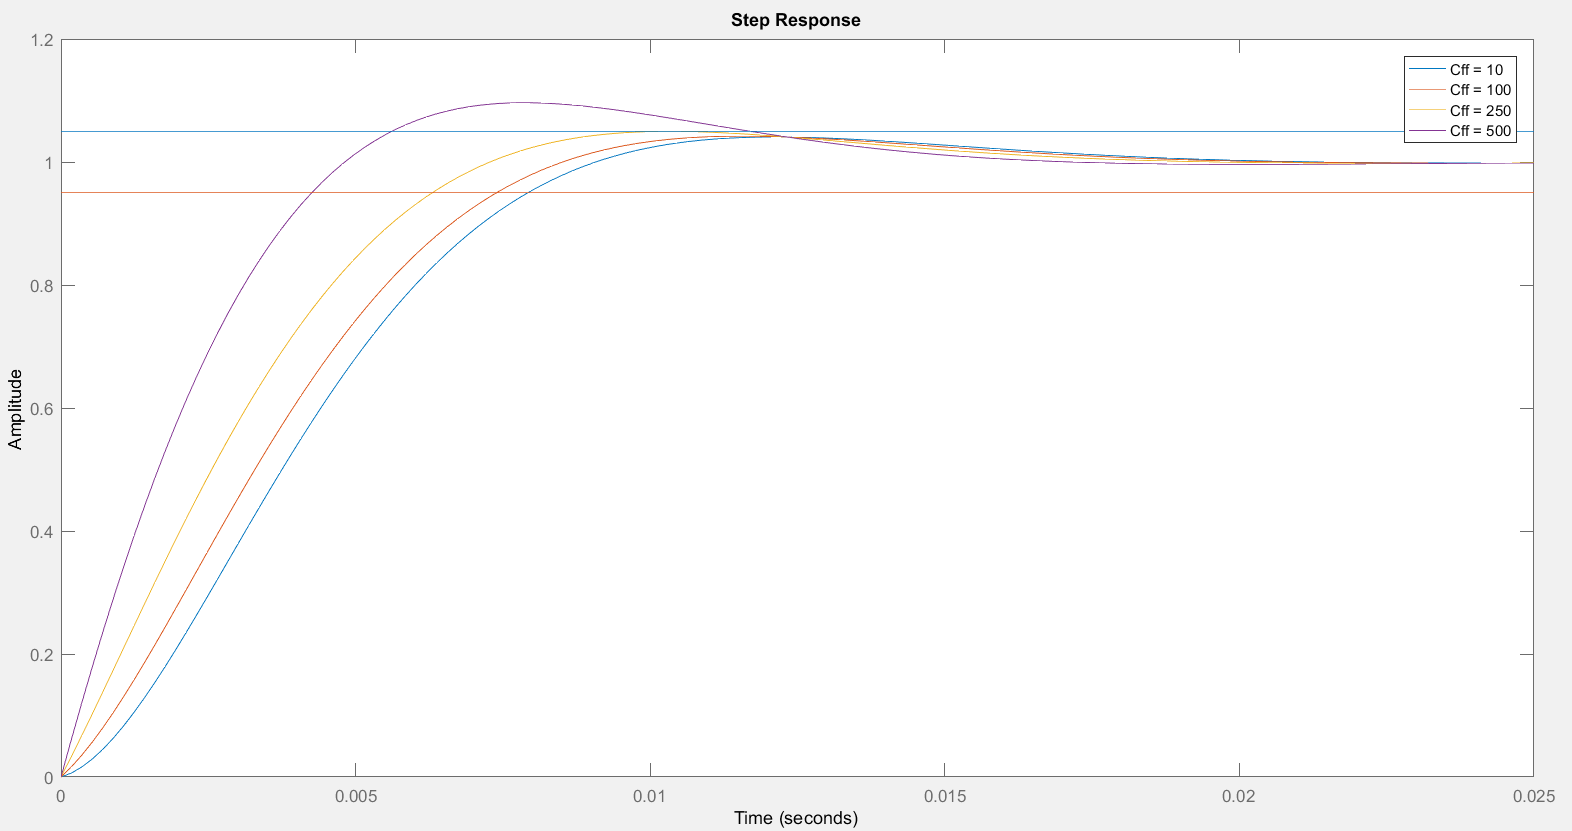
\includegraphics[width=.9\linewidth]{ann_03_a.png}

\vspace{1cm}

Zoom

\vspace{1cm}

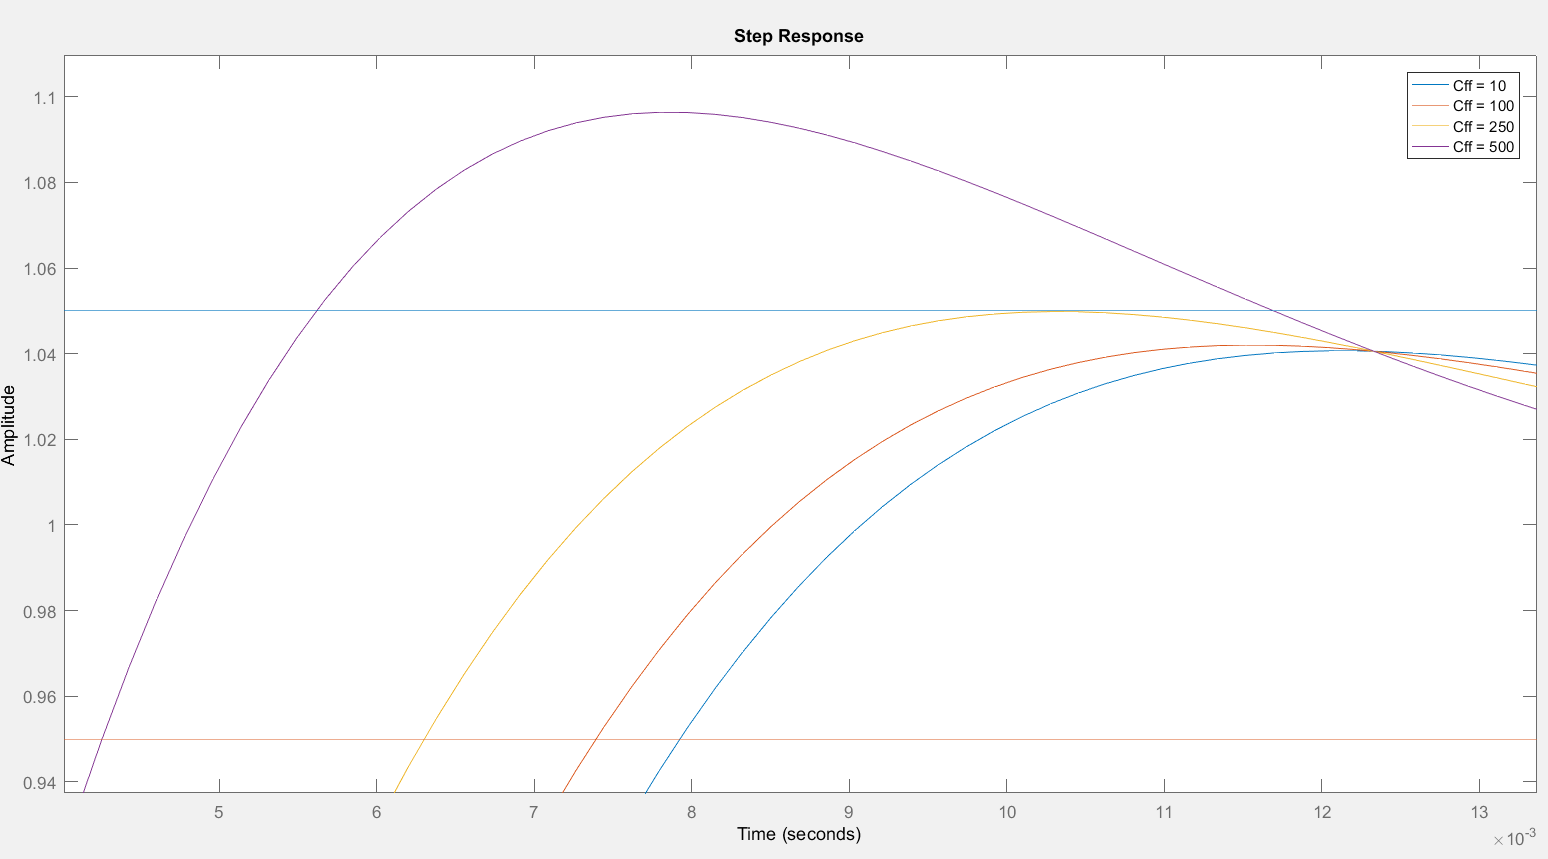
\includegraphics[width=.9\linewidth]{ann_03_b.png}
\end{center}


\section*{Annexe 4 -- Évolution simulée des grandeurs du bras}
\begin{center}
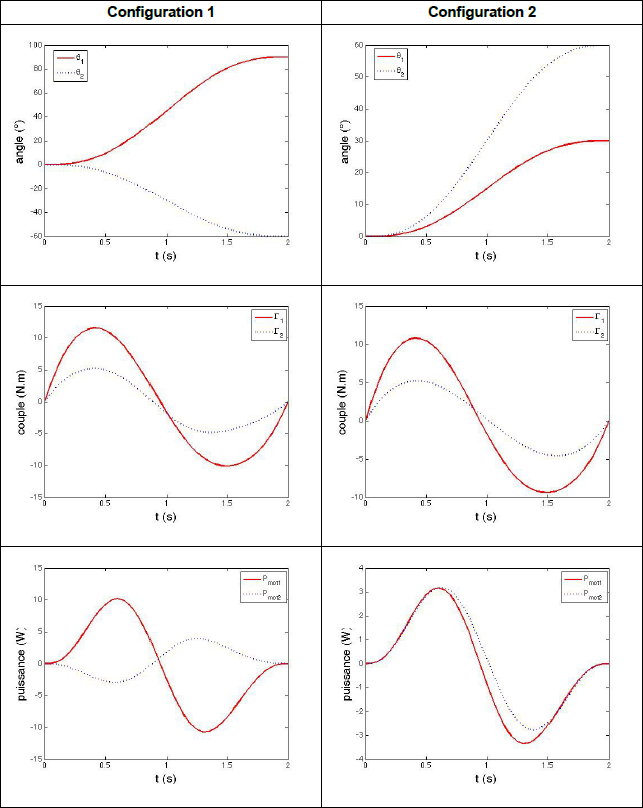
\includegraphics[width=.95\linewidth]{ann_04.png}
\end{center}


\section*{Annexe 5 -- Catalogue de moto-réducteurs}
\begin{center}
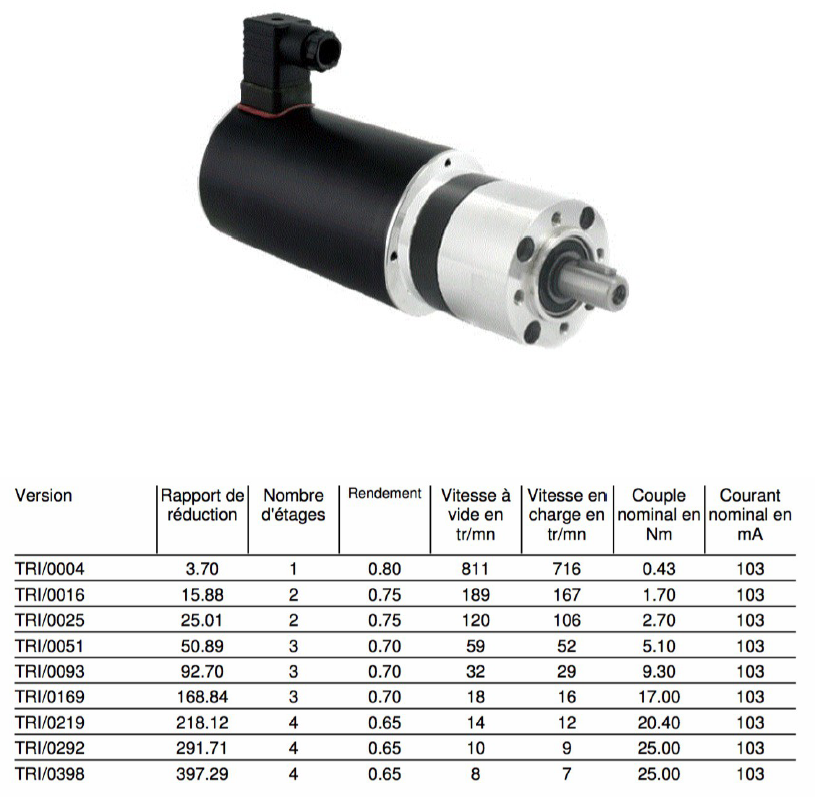
\includegraphics[width=.8\linewidth]{ann_05.png}
\end{center}



%
%\newpage
%\renewcommand{\repExo}{Cy_01_Ch_02_Colle_02_Cisaille}
%\graphicspath{{\repStyle/png/}{\repRel/PSI_Cy_01_ModelisationSystemes/Ch_02_RevisionsSLCI/\repExo/images/}}
%\input{\repRel/PSI_Cy_01_ModelisationSystemes/Ch_02_RevisionsSLCI/\repExo/\repExo.tex}
%
%\newpage
%\mbox{}
%\newpage
%
%\renewcommand{\repExo}{Cy_01_Ch_02_Colle_03_PorteOutil}
%\graphicspath{{\repStyle/png/}{\repRel/PSI_Cy_01_ModelisationSystemes/Ch_02_RevisionsSLCI/\repExo/images/}}
%\input{\repRel/PSI_Cy_01_ModelisationSystemes/Ch_02_RevisionsSLCI/\repExo/\repExo.tex}

\end{document}



